% ============================================================
% MCTS-Based Automated Flowsheet Synthesis — Report 1
% Focus: MDP formulation, unit-op models, MCTS algorithm,
%     separation metrics, multi-condition case study.
% PUCT, Beta regression, and progressive widening are
% deferred to Report 2.
% ============================================================

\documentclass[11pt,a4paper]{article}

% ---------- typography & layout ----------
\usepackage[T1]{fontenc}
\usepackage[utf8]{inputenc}
\usepackage{lmodern}
\usepackage{microtype}
\usepackage[margin=2.5cm]{geometry}
\usepackage{setspace}
\onehalfspacing

% ---------- mathematics ----------
\usepackage{amsmath,amssymb,amsfonts,amsthm}
\usepackage{mathtools}
\usepackage{bm}

% ---------- tables ----------
\usepackage{booktabs}
\usepackage{array}
\usepackage{multirow}
\usepackage{tabularx}

% ---------- algorithms ----------
\usepackage[ruled,linesnumbered,vlined]{algorithm2e}
\SetKwInput{KwInput}{Input}
\SetKwInput{KwOutput}{Output}

% ---------- figures ----------
\usepackage{graphicx}
\usepackage{xcolor}
\usepackage{tikz}
\usetikzlibrary{arrows.meta,shapes.geometric,positioning,calc}

% ---------- references & links ----------
\usepackage[numbers,sort&compress]{natbib}
\usepackage[colorlinks=true,linkcolor=blue!60!black,
      citecolor=green!50!black,urlcolor=blue!70!black]{hyperref}

% ---------- misc ----------
\usepackage{enumitem}
\usepackage{caption}
\usepackage{rotating}
\usepackage{float}
\usepackage{subcaption}
\usepackage{cleveref}

% ---------- theorem environments ----------
\theoremstyle{definition}
\newtheorem{definition}{Definition}[section]
\theoremstyle{plain}
\newtheorem{proposition}{Proposition}[section]
\newtheorem{remark}{Remark}[section]

% ---------- custom commands ----------
\newcommand{\StreamState}{\texttt{StreamState}}
\newcommand{\SearchState}{\texttt{SearchState}}
\newcommand{\MCTSConfig}{\texttt{MCTSConfig}}
\newcommand{\ProcessGraph}{\texttt{ProcessGraph}}
\newcommand{\R}{\mathbb{R}}
\newcommand{\calC}{\mathcal{C}}
\newcommand{\calA}{\mathcal{A}}
\newcommand{\calX}{\mathcal{X}}
\newcommand{\calT}{\mathcal{T}}
\newcommand{\calM}{\mathcal{M}}
\newcommand{\calK}{\mathcal{K}}
\newcommand{\norm}[1]{\left\|#1\right\|}
\newcommand{\abs}[1]{\left|#1\right|}
\DeclareMathOperator*{\argmax}{arg\,max}
\DeclareMathOperator*{\argmin}{arg\,min}

% ============================================================
\begin{document}

\title{\textbf{MCTS-Based Automated Flowsheet Synthesis\\
for Multicomponent Hydrocarbon Separation}\\[6pt]
\large Report~1: Foundations, Unit-Operation Models,
and Multi-Condition Case Study}

\author{
 Oliwer \'{S}liczniuk\\[2pt]
}

\date{\today}

\maketitle
\tableofcontents
\newpage

% ============================================================
\begin{abstract}
Process synthesis — the task of selecting and sequencing unit operations to transform a feed mixture into desired products — is a combinatorial search problem whose solution space grows exponentially with the number of components and unit types. This report presents a Monte~Carlo Tree Search (MCTS) framework for automated flowsheet generation applied to multicomponent hydrocarbon separation.

Rather than relying on heuristics or full enumeration, the algorithm incrementally builds candidate flowsheets by selecting from a thermodynamically constrained set of unit operations: heat exchangers, compressors, pumps, valves, isothermal flash drums, and shortcut distillation columns. Transitions are evaluated using fast simplified models — principally the Fenske--Underwood--Gilliland (FUG) shortcut method together with a Peng--Robinson equation-of-state thermo backend — that are cheap enough to support thousands of evaluations per search run. Separation quality is quantified by a mutual-information metric that measures how well the outlet stream slate resolves the feed composition, yielding a penalty-free separation score $S_{\mathrm{norm}} \in [0,1]$.

The framework is evaluated in a pilot study on nine chemical systems spanning three to five components, including a primary five-component CO$_2$/NGL mixture under five feed conditions (50--200\,kPa, varying compositions). With a pilot budget of 3 seeds $\times$ 1\,500 iterations per run (123 runs total), the search achieves an 86.7\,\% success rate on the primary system and correctly diagnoses five other systems as structurally infeasible or budget-limited. The report details the Markov decision process (MDP) formulation, all unit-operation governing equations, the MCTS algorithm with domain-specific adaptations, and the complete experimental results.
\end{abstract}

% ============================================================
\section{Introduction}
\label{sec:introduction}

% ---- 1.1 Motivation ----------------------------------------
\subsection{Process synthesis as a combinatorial search problem}

The design of chemical separation sequences involves selecting a topology — a network of unit operations connected by material streams — that transforms a feed mixture into a set of product streams meeting purity and recovery specifications. For a mixture containing $n_c$ components, the number of distinct distillation sequences alone is $\frac{(2(n_c-1))!}{(n_c-1)!\,n_c!}$ (the Catalan number $C_{n_c-1}$ for binary split trees), which exceeds one million for $n_c = 15$ ($C_{14} = 2{,}674{,}440$). When heat exchange, pressure manipulation, and flash separation are added alongside distillation, and when operating conditions such as column pressure and reflux ratio become continuous decision variables, complete enumeration is computationally intractable.

Classical approaches to process synthesis fall broadly into three categories. \emph{Heuristic methods} apply rules of thumb — for example, ``remove the most volatile component first'' or ``avoid overly large recycle streams'' — that capture engineering intuition but do not optimize an objective function and can miss non-obvious optima. \emph{Superstructure optimization} embeds all candidate topologies into a single mixed-integer nonlinear program (MINLP), which is guaranteed to find the global optimum but requires a fixed superstructure defined in advance and suffers from combinatorial explosion of binary topology variables. \emph{Stochastic search methods} — including simulated annealing, genetic algorithms, and tabu search — explore the topology space without requiring a fixed superstructure, but do not learn systematically from evaluated candidates.

This work adopts a fourth paradigm: \emph{tree search with online learning}, in which an asymmetric search tree is grown by directing exploration toward promising regions of the topology space based on rewards accumulated from previously evaluated candidates.

\subsection{Why MCTS is suited to flowsheet generation}

Monte~Carlo Tree Search (MCTS) \citep{coulom2006, kocsis2006} was developed for two-player games but has since been applied to single-agent sequential decision problems including program synthesis, molecular design, and combinatorial optimization. Three properties make it particularly suited to automated process synthesis.

\begin{enumerate}[label=(\roman*)]
 \item \textbf{Anytime behaviour.} MCTS can be stopped at any iteration budget and returns the best solution found so far. The quality of that solution improves monotonically with iteration count, so the algorithm adapts to available computational resources without structural modification.

 \item \textbf{Asymmetric tree growth.} Unlike full enumeration or uniform random search, MCTS allocates more evaluations to branches that have historically yielded high rewards, exploiting structure in the search space while maintaining a finite exploration budget on under-visited alternatives.

 \item \textbf{No gradient requirement.} The reward function is evaluated on terminal flowsheet states produced by thermodynamic models. These models are generally non-differentiable with respect to discrete topology choices. MCTS operates entirely on scalar reward values and requires no gradient information.
\end{enumerate}

\subsection{Architecture overview}

The framework operates in two tiers.

\textbf{Tier~1 (MCTS with simplified models).} Candidate flowsheets are generated and evaluated using fast simplified unit models written in pure Python against a Peng--Robinson EOS thermo backend (\texttt{thermo} library). A single flowsheet evaluation requires $O(10)$ flash calculations, each taking $O(1\,\mathrm{ms})$, so 5\,000 MCTS iterations complete in approximately two minutes.

\textbf{Tier~2 (DWSIM rigorous simulation).} Promising topologies identified by MCTS are translated to a DWSIM flowsheet and solved with the full rigorous equation-of-state solver, multi-stage column models, and real utility specifications. Tier~2 provides the final design validation and is outside the scope of this report.

\subsection{Scope of this report}

This report covers:
\begin{itemize}
 \item The MDP formulation of the flowsheet synthesis problem
  (Section~\ref{sec:mdp});
 \item Governing equations of all simplified unit-operation
  models (Section~\ref{sec:units});
 \item Separation quality metrics and the reward function
  (Section~\ref{sec:reward});
 \item The MCTS algorithm and all project-specific
  adaptations (Section~\ref{sec:mcts});
 \item Experimental results on a five-component hydrocarbon
  mixture under five feed conditions
  (Sections~\ref{sec:setup}--\ref{sec:results}).
\end{itemize}

Learned PUCT priors, Beta regression, and the self-improvement
pipeline are deferred to Report~2.

% ============================================================
\section{Problem Formulation as a Finite-Horizon MDP}
\label{sec:mdp}

\subsection{Material stream state}

A material stream is characterised by its thermodynamic and
compositional state
\begin{equation}
 s = (I,\; T,\; P,\; F,\; \bm{z},\; H),
 \label{eq:stream_state}
\end{equation}
where $I$ is an implementation-level identifier, $T$~[K] is temperature, $P$~[Pa] is pressure, $F$~[mol/s] is total molar flow, $\bm{z} \in \R^{n_c}$ is the mole-fraction vector over component set $\calC = \{1,\ldots,n_c\}$, and $H$ is a discrete lineage record tracking the sequence of unit operations that produced the stream. The composition vector lies on the probability simplex:

\begin{equation}
 \sum_{i \in \calC} z_i = 1, \qquad z_i \geq 0.
\end{equation}

In the codebase this object is \StreamState{}. The identifier $I$ is used for display and stream tracking but is not a fundamental chemical property; all identity and similarity computations are based on thermodynamic state and lineage, not on generated stream names.

\subsection{Search state}

At MCTS depth $t$ the complete search state is

\begin{equation}
 X_t = (O_t,\; P_t,\; A_t,\; D_t,\; N_t,\; E_t,\; G_t).
\end{equation}

\begin{table}[ht]
\centering
\caption{Components of the search state $X_t$ (\SearchState{}).}
\label{tab:search_state}
\begin{tabularx}{\linewidth}{@{}cll X@{}}
\toprule
Symbol & Type & Codebase object & Description \\
\midrule
$O_t$ & set & \texttt{set[StreamState]} &
 Open material streams available for further processing \\
$P_t$ & set & \texttt{set[ProductAssignment]} &
 Accepted product stream assignments \\
$A_t = (a_0,\ldots,a_{t-1})$ & sequence & \texttt{list[UnitAction]} &
 Actions applied to reach the current state \\
$D_t$ & float & --- &
 Accumulated absolute duty / shaft-work proxy [W] \\
$N_t$ & float & --- &
 Accumulated theoretical stage count across all columns \\
$E_t$ & tuple & \texttt{tuple[str]} &
 Non-fatal error messages along the current path \\
$G_t$ & graph & \ProcessGraph{} &
 Directed process graph storing topology and stream metadata \\
\bottomrule
\end{tabularx}
\end{table}

The open-stream set $O_t$ is central to the search: after any splitting operation (flash, distillation), the flowsheet has multiple outlet branches and the search may continue on any branch. Accepting a product removes a stream from $O_t$ and adds it to $P_t$.

\subsection{Flowsheets as directed process graphs}
\label{sec:process_graph}

The natural mathematical representation of a candidate flowsheet is a directed process graph

\begin{equation}
 G_t = (V_t^S,\; V_t^U,\; E_t^G,\; \lambda_t),
\end{equation}

where $V_t^S$ contains material-stream nodes, $V_t^U$ contains unit-operation nodes, $E_t^G$ contains directed edges (stream-to-unit and unit-to-stream), and $\lambda_t$ stores node labels (thermodynamic state, unit kind, edge roles). Three fundamental graph motifs appear:

\medskip
\noindent\textit{One-inlet, one-outlet unit operation:}

\begin{equation}
 s_{\mathrm{in}} \;\longrightarrow\; u_k(\theta)
 \;\longrightarrow\; s_{\mathrm{out}}.
\end{equation}

\noindent\textit{Splitting unit (flash, distillation column):}

\begin{equation}
 s_{\mathrm{in}} \;\longrightarrow\; u_k(\theta)
 \;\longrightarrow\; \{s_{\mathrm{out},1},\; s_{\mathrm{out},2}\}.
\end{equation}

\noindent\textit{Recycle mixer (two inlets, one outlet):}

\begin{equation}
 \{s_{\mathrm{feed}},\; s_{\mathrm{recycle}}\}
 \;\longrightarrow\; u_{\mathrm{mix}}
 \;\longrightarrow\; s_{\mathrm{mix}}.
\end{equation}

The graph is implemented as a first-class immutable object \ProcessGraph{} stored directly on every \SearchState{} and grown incrementally by atomic graph-append operations at each action. Graph identity, topology hashing, result clustering, and future DWSIM translation all operate on this explicit representation.

\subsection{MDP formulation}
\label{sec:mdp_formal}

The flowsheet generation problem is formalised as a finite-horizon Markov decision process

\begin{equation}
 \calM = (\calX,\; \calA,\; \calT,\; R,\; H_{\max}),
\end{equation}

where:

\begin{itemize}
 \item $\calX$ is the set of all reachable process states;
 \item $\calA(X)$ is the state-dependent valid action set;
 \item $\calT : \calX \times \calA \to \calX$ is the
  deterministic transition operator induced by the simplified
  unit models;
 \item $R : \calX \to \R$ is the reward function evaluated at
  terminal or leaf states;
 \item $H_{\max}$ is the maximum search depth.
\end{itemize}

\begin{remark}[Markov property]
 Each action consumes exactly one open stream and produces one or two outlet streams. The full thermodynamic state of those outlets is determined entirely by the inlet stream state and the action parameters. Path-dependent features such as step count $\abs{A_t}$ and accumulated duty $D_t$ are included explicitly in $X_t$, so the transition $\calT$ is Markov in $X_t$.
\end{remark}

\subsection{Action representation and valid action set}
\label{sec:actions}

Each action is a tuple

\begin{equation}
 a_t = (k,\; I_{\mathrm{in}},\; \theta),
\end{equation}

where $k$ is the unit-operation kind, $I_{\mathrm{in}}$ identifies the consumed open stream, and $\theta$ contains unit-specific parameters (temperature delta, pressure ratio, key-component pair, recovery fractions, etc.). The action kinds implemented are: heat exchange (\texttt{hx}), isothermal flash (\texttt{flash}), compressor, pump, valve, shortcut distillation (\texttt{distillation}), recycle mixer (\texttt{recycle}), and product acceptance (\texttt{accept}).

The complete valid action set is

\begin{equation}
 \calA(X_t)
 = \bigcup_{s \in \tilde{O}_t}
  \calA_s(X_t, s;\; \omega),
\end{equation}

where $\omega$ denotes the configuration object \MCTSConfig{} and $\tilde{O}_t \subseteq O_t$ is the active stream subset after stream-priority gating (Section~\ref{sec:priority}). Feasibility constraints on individual action kinds are:

\medskip
\noindent\textit{Temperature bounds (heat exchange):}

\begin{equation}
 T_{\min} \;\leq\; T + \Delta T \;\leq\; T_{\max}.
\end{equation}

\noindent\textit{Pressure bounds (compressor, pump, valve):}

\begin{equation}
 P_{\min} \;\leq\; P_{\mathrm{out}} \;\leq\; P_{\max}.
\end{equation}

\noindent\textit{Minimum retained flow (all actions):}

\begin{equation}
 F \;\geq\; F_{\min}.
\end{equation}

\noindent\textit{Lineage constraints:}

\begin{equation}
 n_{\mathrm{flash}}(s) < N_{\mathrm{flash,max}},
 \qquad
 n_{\mathrm{dist}}(s) < N_{\mathrm{dist,max}},
 \qquad
 n_{\mathrm{rec}}(s) < N_{\mathrm{rec,max}}.
\end{equation}

\noindent\textit{Global distillation cap:}

\begin{equation}
 \sum_{a \in A_t} \mathbf{1}[k(a) = \mathrm{distillation}]
 \;<\; N_{\mathrm{dist,total,max}}.
\end{equation}

\subsubsection{Distillation key-pair enumeration}

For distillation actions the valid key-pair set depends on the relative-volatility ordering of the components in stream $s$. Let the components be sorted in decreasing volatility order so that $\alpha_1 \geq \alpha_2 \geq \cdots \geq \alpha_{n_c}$. In \emph{adjacent mode} (used in all experiments), only consecutive volatility pairs are proposed:

\begin{equation}
 \calK_{\mathrm{adj}} = \{(c_j,\; c_{j+1})
 : j = 1,\ldots,n_c-1\}.
 \label{eq:adj_key_pairs}
\end{equation}

This produces exactly $n_c - 1$ key-pair proposals per stream, guaranteeing complete coverage of all adjacent volatility boundaries without redundant or physically implausible skipped-key splits.

\subsubsection{Phase gates for pressure-changing actions}

A \emph{compressor gate} suppresses all compressor actions for streams with vapor fraction below a configured minimum ($\mathrm{VF}_{\mathrm{in}} < \phi_{\min}^{\mathrm{comp}}$), routing such streams to a pump instead. A \emph{pump gate} suppresses all pump actions for streams with vapor fraction above a configured maximum ($\mathrm{VF}_{\mathrm{in}} > \phi_{\max}^{\mathrm{pump}}$, default $10^{-6}$), preventing pump actions on gaseous or two-phase streams that would immediately fail at apply time.

\subsection{Stream-priority gating}
\label{sec:priority}

Before generating actions, streams can be filtered by a flow-weighted composition entropy metric. For stream $s$ with mole-fraction vector $\bm{z}_s$, the normalised Shannon entropy is

\begin{equation}
 H_{\mathrm{norm}}(\bm{z}_s)
 = -\frac{1}{\ln\abs{\calC_s}}
  \sum_{i \in \calC_s} z_{s,i} \ln z_{s,i},
\end{equation}

where $\calC_s$ is the set of components with mole fraction above a minimum threshold. The stream priority is

\begin{equation}
 \pi(s;\; s_0)
 = \frac{F_s}{F_0}\, H_{\mathrm{norm}}(\bm{z}_s)
 \;\in\; [0,1],
\end{equation}

where $F_0$ is the feed molar flow. This metric is large only for streams that are both materially significant and compositionally mixed. The active stream subset is either

\begin{equation}
 \tilde{O}_t
 = \{s \in O_t : \pi(s;\; s_0) \geq \pi_{\min}\}
 \quad\text{(threshold mode)},
\end{equation}

or the top-$k$ streams by priority (top-$k$ mode). Accept actions are always generated regardless of stream priority, because the near-pure streams that should be accepted are exactly those with low priority score.

\subsection{State transition}

Given an action $a_t = (k, I_{\mathrm{in}}, \theta)$, the next state is

\begin{equation}
 X_{t+1} = \calT(X_t, a_t).
\end{equation}

For a unit operation consuming one stream and producing one or more outlets, the open-stream update is

\begin{equation}
 O_{t+1}
 = \bigl(O_t \setminus \{s_{\mathrm{in}}\}\bigr)
  \cup \mathcal{U}_k(s_{\mathrm{in}}, \theta),
\end{equation}

where $\mathcal{U}_k$ is the simplified model for unit kind $k$. For a product-acceptance action:

\begin{equation}
 P_{t+1} = P_t \cup \{(\rho,\; s_{\mathrm{in}})\},
 \qquad
 O_{t+1} = O_t \setminus \{s_{\mathrm{in}}\}.
\end{equation}

The accumulated duty and stage count are updated as

\begin{equation}
 D_{t+1} = D_t + \Delta D_k, \qquad
 N_{t+1} = N_t + \Delta N_k,
\end{equation}

where $\Delta N_k > 0$ only for distillation actions.

% ============================================================
\section{Simplified Unit-Operation Models}
\label{sec:units}

The unit models used in the search are intentionally simplified. Their purpose is to provide a fast thermodynamic approximation that can distinguish promising from poor topologies within milliseconds per evaluation, not to replace rigorous DWSIM simulation. All models call a Peng--Robinson EOS flash backend from the \texttt{thermo} library to evaluate enthalpies, entropies, $K$-values, and vapor fractions.

\subsection{Heat exchange}
\label{sec:hx}

The decision variable is a temperature increment $\Delta T$. The outlet conditions are

\begin{equation}
 T_{\mathrm{out}} = T_{\mathrm{in}} + \Delta T,
 \qquad
 P_{\mathrm{out}} = P_{\mathrm{in}}.
\end{equation}

The duty is the enthalpy difference at constant pressure:

\begin{equation}
 Q = F \bigl[\hat{h}(T_{\mathrm{out}},\, P_{\mathrm{in}},\,
  \bm{z}) - \hat{h}(T_{\mathrm{in}},\, P_{\mathrm{in}},\,
  \bm{z})\bigr],
\end{equation}

where $\hat{h}$ is the molar enthalpy returned by the thermo provider. The accumulated duty increases by the absolute value: $D_{t+1} = D_t + \abs{Q}$.

\paragraph{Phase-boundary targets.}
In addition to a fixed $\Delta T$ grid, the heat-exchanger action generator can target thermodynamically meaningful phase boundaries. A target vapor fraction $\phi^\star \in \{0, 1, \phi_{\mathrm{partial}}\}$ specifies the desired outlet phase state; the corresponding outlet temperature $T^\star$ is obtained from a constant-pressure PVF flash:

\begin{equation}
 (P_{\mathrm{in}},\; \phi^\star,\; \bm{z})
 \;\xrightarrow{\mathrm{PVF\,flash}}\;
 T^\star,
 \qquad \Delta T = T^\star - T_{\mathrm{in}}.
\end{equation}

Actions with $\abs{\Delta T} < 0.5\,\mathrm{K}$ are discarded; deduplication tolerance is $0.1\,\mathrm{K}$.

\subsection{Compressor}
\label{sec:compressor}

The compressor raises the pressure of a vapor-phase stream. For a pressure-ratio action, $P_{\mathrm{out}} = r P_{\mathrm{in}}$ with $r > 1$; for a delta-pressure action, $P_{\mathrm{out}} = P_{\mathrm{in}} + \Delta P$. The shaft work is computed from inlet and isentropic-outlet enthalpies:

\begin{equation}
 W_s = F \cdot \frac{\hat{h}(S_{\mathrm{in}},\,
  P_{\mathrm{out}},\, \bm{z}) - \hat{h}(T_{\mathrm{in}},\,
  P_{\mathrm{in}},\, \bm{z})}{\eta_{\mathrm{is}}\,
  \eta_{\mathrm{mech}}},
\end{equation}

where $S_{\mathrm{in}} = S(T_{\mathrm{in}}, P_{\mathrm{in}}, \bm{z})$ is the inlet molar entropy and $\hat{h}(S, P, \bm{z})$ is the enthalpy at fixed entropy $S$ and pressure $P$ (the isentropic outlet). $D_{t+1} = D_t + \abs{W_s}$.

\paragraph{Dew-pressure target.}
The compressor can also target the minimum outlet pressure at which isentropic compression causes condensation onset:

\begin{equation}
 P^\star = \inf\!\left\{P \in [P_{\mathrm{in}},\; P_{\max}]
 : \mathrm{VF}(S_{\mathrm{in}},\, P,\, \bm{z}) < 1\right\},
\end{equation}

located by bisection with relative precision $10^{-6}$.

\subsection{Pump}
\label{sec:pump}

The pump model mirrors the compressor but applies to liquid-phase streams and uses the same isentropic-work equation. The pump gate rejects any inlet with $\mathrm{VF}_{\mathrm{in}} > \phi_{\max}^{\mathrm{pump}} \approx 10^{-6}$.

\paragraph{Bubble-pressure target.}
The pump can target the pressure at which the liquid stream first reaches the bubble line at the inlet temperature:

\begin{equation}
 (T_{\mathrm{in}},\; 0,\; \bm{z})
 \;\xrightarrow{\mathrm{TVF\,flash}}\;
 P^\star.
\end{equation}

A pump action with ratio $r = P^\star / P_{\mathrm{in}}$ is generated when $P^\star > P_{\mathrm{in}}$.

\subsection{Valve}
\label{sec:valve}

The valve reduces pressure via isenthalpic expansion: $P_{\mathrm{out}} < P_{\mathrm{in}}$, $H_{\mathrm{out}} = H_{\mathrm{in}}$. The duty is zero.

\paragraph{Bubble-pressure target.}
The valve targets the highest outlet pressure at which isenthalpic expansion first produces a vapor phase:

\begin{equation}
 P^\star = \sup\!\left\{P \in [P_{\min},\; P_{\mathrm{in}}]
 : \mathrm{VF}(H_{\mathrm{in}},\, P,\, \bm{z}) > 0\right\}.
\end{equation}

\subsection{Flash separation}
\label{sec:flash}

The flash model performs a pressure-temperature flash at the inlet conditions:

\begin{equation}
 \Phi(T, P, \bm{z})
 \;\mapsto\;
 (\beta,\; \bm{z}^V,\; \bm{z}^L),
\end{equation}

where $\beta$ is the vapor fraction. A flash action produces two outlets only when the result is two-phase ($0 < \beta < 1$). The outlet flows are $F^V = \beta F$ and $F^L = (1-\beta)F$; outlets below $F_{\min}$ are dropped.

\paragraph{Flash drum duty proxy.}
For an isothermal-isobaric flash drum the thermodynamic duty at the system boundary is formally zero. As a useful proxy for the separation energy cost, the implementation uses the latent heat of the vapor fraction:

\begin{equation}
 Q_{\mathrm{flash}}
 = F \cdot \beta \cdot \max\!\bigl(0,\;
  h^V - h^L\bigr),
\end{equation}

where $h^V$ and $h^L$ are the molar enthalpies of the equilibrium vapor and liquid phases at $(T, P)$. This is always non-negative and is accumulated into $D_t$.

\subsection{Shortcut distillation — FUG method}
\label{sec:distillation}

Shortcut distillation uses the Fenske--Underwood--Gilliland (FUG) calculation to estimate whether a proposed light-key/heavy-key separation is plausible and to obtain estimates of the number of theoretical stages and reflux ratio.

Let $\mathrm{LK}$ and $\mathrm{HK}$ denote the light and heavy key components with specified distillate recoveries $r_{\mathrm{LK}}$ and $r_{\mathrm{HK}}$, satisfying $0 < r_{\mathrm{HK}} < r_{\mathrm{LK}} < 1$.

\subsubsection{Relative volatilities}
\label{sec:relVol}

Relative volatilities are estimated from a PVF flash at the stream pressure and $\mathrm{VF} = 0.5$, giving $K$-values $K_i = y_i / x_i$:

\begin{equation}
 \alpha_i = \frac{K_i}{K_{\mathrm{HK}}},
 \qquad \alpha_{\mathrm{HK}} = 1.
\end{equation}

\subsubsection{Fenske minimum stages}
\label{sec:fenske}

Key molar flows to distillate and bottoms:
\begin{equation}
 n_{\mathrm{LK}}^D = r_{\mathrm{LK}}\, n_{\mathrm{LK}}^F,
 \quad
 n_{\mathrm{HK}}^D = r_{\mathrm{HK}}\, n_{\mathrm{HK}}^F,
 \quad
 n_{\mathrm{LK}}^B = (1-r_{\mathrm{LK}})\, n_{\mathrm{LK}}^F,
 \quad
 n_{\mathrm{HK}}^B = (1-r_{\mathrm{HK}})\, n_{\mathrm{HK}}^F.
\end{equation}

The Fenske minimum stage count is:

\begin{equation}
 N_{\min}
 = \frac{\ln\!\left[
   \dfrac{n_{\mathrm{LK}}^D / n_{\mathrm{HK}}^D}{
      n_{\mathrm{LK}}^B / n_{\mathrm{HK}}^B}
  \right]}{\ln(\alpha_{\mathrm{LK}})}.
 \label{eq:fenske}
\end{equation}

\paragraph{Non-key distribution.}
For each non-key component $i$, the Fenske distribution ratio is

\begin{equation}
 d_i = \frac{n_{\mathrm{HK}}^D}{n_{\mathrm{HK}}^B}
    \cdot \alpha_i^{N_{\min}},
\end{equation}
giving $n_i^D = n_i^F\, d_i / (1 + d_i)$.

\subsubsection{Underwood minimum reflux}
\label{sec:underwood}

The Underwood root $\theta$ satisfying $\alpha_{\mathrm{HK}} < \theta < \alpha_{\mathrm{LK}}$ is found from:

\begin{equation}
 \sum_{i \in \calC}
 \frac{\alpha_i\, z_i}{\alpha_i - \theta} = 1 - q,
 \label{eq:underwood_root}
\end{equation}

where $q = 1 - \mathrm{VF}_{\mathrm{in}}$ is the liquid fraction of the feed. The minimum reflux ratio is then

\begin{equation}
 R_{\min}
 = \sum_{i \in \calC}
  \frac{\alpha_i\, x_i^D}{\alpha_i - \theta} - 1.
 \label{eq:rmin}
\end{equation}

\paragraph{Adjacency requirement.}
The Underwood feed function $f(\theta) = \sum_i \alpha_i z_i / (\alpha_i - \theta)$ has a pole at $\theta = \alpha_j$ for every component $j$. Within a pole-free interval $(\alpha_{\mathrm{HK}}, \alpha_{\mathrm{LK}})$, $f$ is strictly monotone and Eq.~\eqref{eq:underwood_root} has a unique root — but only when no component $j$ satisfies $\alpha_{\mathrm{HK}} < \alpha_j < \alpha_{\mathrm{LK}}$ (the Mazzotti adjacency condition). A distributing component in the interval creates an additional pole, meaning the single-root formula underestimates $R_{\min}$. The implementation therefore rejects any non-adjacent key pair by returning \texttt{None} from the Underwood solver, and that pair is excluded from the valid action set.

\begin{remark}[Adjacency and complete separation] 
	For a five-component system with volatility order $\alpha_1 > \cdots > \alpha_5$, the four adjacent pairs $(c_1,c_2), (c_2,c_3), (c_3,c_4), (c_4,c_5)$ are the only pairs that can be represented by a single Underwood root. Any complete separation of all five components into pure products requires at most $n_c - 1 = 4$ adjacent-pair columns. The \texttt{adjacent} key-pair mode in Eq.~\eqref{eq:adj_key_pairs} therefore covers the complete-separation problem exactly.
\end{remark}

\paragraph{Newton--Raphson--bisection solver.}
Within the verified pole-free interval, the function $g(\theta) = f(\theta) - (1-q)$ is smooth, strictly monotone, and has a unique root. The Newton step is

\begin{equation}
 \theta_{k+1} = \theta_k - \frac{g(\theta_k)}{g'(\theta_k)},
 \qquad
 g'(\theta) = \sum_{i \in \calC}
  \frac{\alpha_i\, z_i}{(\alpha_i - \theta)^2} > 0.
\end{equation}

When a Newton step escapes the bracket
$(\alpha_{\mathrm{HK}}, \alpha_{\mathrm{LK}})$, the bracket is tightened and the bisection midpoint is used instead (safe Newton--bisection hybrid). Convergence is declared when $\abs{g(\theta)} < 10^{-12}$, typically in 5--8 iterations from the midpoint starting guess $\theta_0 = (\alpha_{\mathrm{HK}} + \alpha_{\mathrm{LK}})/2$.

\subsubsection{Gilliland stage estimate}
\label{sec:gilliland}

The operating reflux ratio is $R = m_R R_{\min}$ with multiplier $m_R > 1$. Define

\begin{equation}
 X_G = \frac{R - R_{\min}}{R + 1} \in (0,1).
\end{equation}

The Liddle form of the Gilliland correlation gives the stage fraction $Y$:

\begin{equation}
 Y = 1 - \exp\!\left[
  \frac{1 + 54.4\, X_G}{11 + 117.2\, X_G}
  \cdot \frac{X_G - 1}{\sqrt{X_G}}
 \right],
 \label{eq:gilliland_Y}
\end{equation}

and the theoretical stage count is

\begin{equation}
 N = \frac{N_{\min} + Y}{1 - Y}.
 \label{eq:gilliland_N}
\end{equation}

The Gilliland stage estimate $N$ is accumulated into the search state: $N_{t+1} = N_t + N$.

\subsubsection{Product stream temperatures}

The distillate exits a total condenser as a saturated liquid at column pressure $P$. Its temperature $T_D$ is obtained from a PVF flash at $(P, \mathrm{VF}=0, \bm{z}_D)$. The bottoms exits at its bubble point: $T_B$ from $(P, \mathrm{VF}=0, \bm{z}_B)$.

\subsection{Full column energy balance}
\label{sec:energy_balance}

When configuration option \texttt{include\_reboiler\_duty=True}, both condenser and reboiler duties are estimated from a rigorous energy balance using the Peng--Robinson EOS, at the cost of four additional flash evaluations per column.

\paragraph{Control volume and first law.}
Consider a steady-state energy balance around the entire column system (condenser and reboiler included). The first law for an open system at steady state gives:

\begin{equation}
 F_F\, h_F + Q_{\mathrm{reb}}
 = F_D\, h_D + F_B\, h_B + Q_{\mathrm{cond}},
 \label{eq:EB_full}
\end{equation}

where $h_F$, $h_D$, $h_B$ are molar enthalpies and $Q_{\mathrm{reb}}, Q_{\mathrm{cond}} \geq 0$ by convention (positive heat input at reboiler, positive removal at condenser). Rearranging:

\begin{equation}
 Q_{\mathrm{reb}}
 = Q_{\mathrm{cond}}
 + F_D\, h_D + F_B\, h_B - F_F\, h_F.
 \label{eq:reb_from_cond}
\end{equation}

\paragraph{Condenser duty.}
For a total condenser, the overhead vapor flow is $V_{\mathrm{top}} = (R+1) F_D$ with composition $\bm{z}_D$. Fully condensing this vapor to a saturated liquid at column pressure $P$ gives:

\begin{equation}
 Q_{\mathrm{cond}}
 = (R+1)\, F_D\, \lambda_D,
 \qquad
 \lambda_D = h_{\mathrm{vap},D} - h_{\mathrm{liq},D},
\end{equation}

where

\begin{equation}
 h_{\mathrm{liq},D} = \hat{h}(P,\; \mathrm{VF}{=}0,\; \bm{z}_D),
 \qquad
 h_{\mathrm{vap},D} = \hat{h}(P,\; \mathrm{VF}{=}1,\; \bm{z}_D).
\end{equation}

\paragraph{Required flash calls.}

\begin{table}[ht]
\centering
\caption{Four flash evaluations required by the full energy
 balance model.}
\label{tab:flash_calls}
\begin{tabular}{@{}llll@{}}
\toprule
Call & Input & Purpose & Result \\
\midrule
1 & $(T_F,\, P_F,\, \bm{z}_F)$ & Feed molar enthalpy & $h_F$ \\
2 & $(P,\, \mathrm{VF}{=}0,\, \bm{z}_D)$ & Distillate bubble-point enthalpy & $h_{\mathrm{liq},D} = h_D$ \\
3 & $(P,\, \mathrm{VF}{=}1,\, \bm{z}_D)$ & Distillate dew-point enthalpy & $h_{\mathrm{vap},D}$ \\
4 & $(P,\, \mathrm{VF}{=}0,\, \bm{z}_B)$ & Bottoms bubble-point enthalpy & $h_{\mathrm{liq},B} = h_B$ \\
\bottomrule
\end{tabular}
\end{table}

\paragraph{Reboiler duty.}
Substituting into Eq.~\eqref{eq:reb_from_cond}:

\begin{equation}
 Q_{\mathrm{reb}}
 = (R+1)\, F_D\, \lambda_D
 + \underbrace{F_D\, h_D + F_B\, h_B
  - F_F\, h_F}_{\Delta H_{\mathrm{streams}}}.
 \label{eq:Q_reb}
\end{equation}

$\Delta H_{\mathrm{streams}} > 0$ when the combined product enthalpy exceeds the feed enthalpy (typical above-ambient columns), giving $Q_{\mathrm{reb}} > Q_{\mathrm{cond}}$. For cryogenic columns where products are colder than the feed, $\Delta H_{\mathrm{streams}} < 0$ and $Q_{\mathrm{reb}} < Q_{\mathrm{cond}}$; the reboiler operates below the condenser duty because the feed itself provides heat to both products. Both cases are handled correctly by the signed energy balance.

\paragraph{Duty accumulation.}
Both duties are accumulated:

\begin{equation}
 D_{t+1} = D_t + \abs{Q_{\mathrm{cond}}} + \abs{Q_{\mathrm{reb}}}.
\end{equation}

Absolute values ensure a non-negative duty increment in the cryogenic regime.

% ============================================================
\section{Separation Quality Metrics and Reward Function}
\label{sec:reward}

\subsection{Purity-recovery metric}
\label{sec:pr_metric}

Let $Y(X) = P_X \cup O_X$ denote the full outlet slate. For each component $i \in \calC'$ with feed fraction $z_i^0 > z_{\min}$, define for outlet stream $y$:

\begin{equation}
 \pi_i(y) = z_{i,y},
 \qquad
 \rho_i(y) = \frac{F_y\, z_{i,y}}{F_0\, z_i^0}.
\end{equation}

The component score is the best purity-recovery product over all outlet streams:

\begin{equation}
 \phi_i(Y) = \max_{y \in Y}
 \bigl[\pi_i(y) \cdot \mathrm{clip}(\rho_i(y), 0, 1)\bigr].
\end{equation}

The total separation score is:

\begin{equation}
 \sigma_{\mathrm{PR}}(X)
 = \sum_{i \in \calC'} \phi_i(Y(X))
 \;\in\; [0,\; \abs{\calC'}].
 \label{eq:sigma_PR}
\end{equation}

\paragraph{Limitation.}
A single mixed stream with positive mole fractions of multiple components can rank first for several components simultaneously, inflating $\sigma_{\mathrm{PR}}$ without achieving genuine separation. The mutual information metric below eliminates this degeneracy by construction.

\subsection{Mutual information separation metric}
\label{sec:mi_metric}

\paragraph{Joint distribution.}
For an outlet slate $Y(X) = \{y_1,\ldots,y_M\}$, define the joint probability of a randomly sampled molecule belonging to component $i$ and residing in stream $k$:

\begin{equation}
 P(C=i,\; K=k)
 = \frac{F_{y_k}\, x_{i,y_k}}{F_0}.
 \label{eq:joint_dist}
\end{equation}

The component marginal recovers the feed mole fraction: $P(C=i) = z_i^0$. The stream marginal is $P(K=k) = F_{y_k}/F_0$.

\paragraph{Mutual information.}
The conditional entropy of component identity given stream membership is:

\begin{equation}
 H(C \mid K)
 = -\sum_k \frac{F_{y_k}}{F_0}
  \sum_{i \in \calC'} x_{i,y_k} \ln x_{i,y_k}.
\end{equation}

The inner sum is the mixing entropy of stream $k$: zero for a pure stream, $H(C)$ for a fully mixed stream. The mutual information is:

\begin{equation}
 I(C;\; K) = H(C) - H(C \mid K),
 \label{eq:MI}
\end{equation}

where $H(C) = -\sum_i z_i^0 \ln z_i^0$ is the feed entropy (fixed for a given feed). $I(C;K) = 0$ when all outlets have feed composition; $I(C;K) = H(C)$ when each component is in its own pure stream.

\paragraph{Equal-weight normalisation.}
The standard formulation weights each component's separation credit by its feed fraction $z_i^0$, so trace components contribute little even when cleanly separated. The equal-weight variant replaces the empirical component marginal $P(C=i) = z_i^0$ with a \emph{uniform prior} $P_{\mathrm{eq}}(C=i) = 1/n_c$, recomputing the mutual information entirely under this prior.

Concretely, the component-flow matrix $A_{ik} = F_k\,x_{i,k}$ is row-normalised to give the outlet-distribution conditional:

\begin{equation}
 P(K = k \mid C = i)
 = \frac{A_{ik}}{\displaystyle\sum_{k'} A_{ik'}}.
\end{equation}

The joint distribution under the uniform prior is $B_{ik} = P_{\mathrm{eq}}(C=i)\,P(K=k\mid C=i)$, with marginal $P_{\mathrm{eq}}(K=k) = \sum_i B_{ik}$. The equal-weight mutual information is then:

\begin{equation}
 I_{\mathrm{eq}}(C;K)
 = \sum_{i,k} B_{ik}
  \ln\!\frac{B_{ik}}{P_{\mathrm{eq}}(C=i)\,P_{\mathrm{eq}}(K=k)}.
\end{equation}

Under the uniform prior the reference entropy is $H_{\mathrm{eq}}(C) = \ln n_c$, giving the score:

\begin{equation}
 \sigma_{\mathrm{MI,eq}}(X)
 = n_c \cdot \frac{I_{\mathrm{eq}}(C;\,K)}{\ln n_c},
 \label{eq:sigma_MI_eq}
\end{equation}

so that each component contributes equally to the score regardless of its feed abundance. The normalised fraction $S_{\mathrm{norm}} = \sigma_{\mathrm{MI,eq}}/n_c \in [0,1]$.

\paragraph{Material-balance robustness.}
The equal-weight implementation avoids explicit material-balance normalisation by construction: only the conditional distributions $P(K=k \mid C=i) = A_{ik}/\sum_{k'} A_{ik'}$ appear in the formula, so absolute outlet flows cancel. Dropped low-flow outlets or recycle-augmented outlets therefore do not distort $I_{\mathrm{eq}}$. Components whose total outlet flow falls below a numerical tolerance are excluded from the valid set; their contribution to $I_{\mathrm{eq}}$ is zero without any special-casing.

\paragraph{Properties.}
\begin{itemize}
 \item \textit{Degeneracy-safe.} A unit operation whose outlet streams have the same component distribution as the feed contributes $P(K=k \mid C=i) \approx P_{\mathrm{eq}}(K=k)$ for all $k$, giving zero KL divergence and zero $I_{\mathrm{eq}}$. Adding a non-separating unit cannot increase the score.
 \item \textit{Equal credit.} Every component with non-zero outlet flow contributes identically to $I_{\mathrm{eq}}$ in a perfect separation, regardless of feed fraction. The equal-weight prior eliminates the bias toward abundant components that is present in the standard (feed-fraction) MI formulation.
 \item \textit{Non-negative.} $I_{\mathrm{eq}} \geq 0$ by the non-negativity of KL divergence; the row normalisation of $A$ guarantees this even when total outlet flow differs from feed flow.
\end{itemize}

\subsection{Reward function}
\label{sec:reward_fn}

In complete-separation mode, the reward is:

\begin{equation}
 R_{\mathrm{base}}(X)
 = \sigma(X)
 - \alpha_u\, \abs{A_t}
 - \alpha_d\, D_t
 - \alpha_N\, N_t
 - 0.5\, \abs{E_t},
 \label{eq:reward_base}
\end{equation}

where $\sigma(X)$ is either $\sigma_{\mathrm{PR}}$ or $\sigma_{\mathrm{MI,eq}}$ according to \texttt{separation\_score\_mode}.

\begin{table}[ht]
\centering
\caption{Reward function penalty terms.}
\label{tab:penalties}
\begin{tabular}{@{}clcc@{}}
\toprule
Symbol & Description & Config field & Default \\
\midrule
$\alpha_u$ & Per-action (unit) penalty & \texttt{unit\_penalty} & 0.01 \\
$\alpha_d$ & Per-watt duty penalty & \texttt{duty\_penalty\_per\_W} & $10^{-5}$ \\
$\alpha_N$ & Per-stage penalty & \texttt{stage\_count\_penalty\_per\_stage} & 0.0 \\
$D_t$ & Accumulated duty [W] & \texttt{total\_abs\_duty\_W} & 0 \\
$N_t$ & Accumulated stages & \texttt{total\_theoretical\_stages} & 0 \\
\bottomrule
\end{tabular}
\end{table}

\paragraph{Reward normalisation.}
To make the UCT exploration coefficient $c$ transferable across problem sizes, rewards are normalised by dividing by $\abs{\calC'}$:

\begin{equation}
 R_{\mathrm{norm}}(X)
 = \frac{R_{\mathrm{base}}(X)}{\abs{\calC'}}.
 \label{eq:reward_norm}
\end{equation}

Because $R_{\mathrm{base}}$ subtracts penalty terms, $R_{\mathrm{norm}}$ can be slightly negative for sequences with large duty or many actions; the upper bound is 1 when $\sigma = \abs{\calC'}$ and all penalties are zero. The penalty-free normalised separation score, which is strictly in $[0,1]$, is:

\begin{equation}
 S_{\mathrm{norm}}(X)
 = \frac{\sigma_{\mathrm{MI,eq}}(X)}{n_c}
 = \frac{I_{\mathrm{eq}}(C;\; K)}{\ln n_c}
 \;\in\; [0, 1].
\end{equation}

\subsection{Terminal conditions}
\label{sec:terminal}

A search state $X_t$ becomes terminal when any of the following hold:

\begin{enumerate}[label=(\roman*)]
 \item $\sigma(X_t) \geq \sigma^\star - \varepsilon_{\mathrm{sep}}$
  (separation threshold reached);
 \item $\abs{A_t} \geq H_{\max}$ (maximum depth);
 \item $O_t = \emptyset$ (no open streams remain).
\end{enumerate}

A stream is excluded from further processing (\textit{auto-closed}) when its dominant-component mole fraction meets the purity threshold $\rho^\star$, reducing the branching factor at near-complete states.

% ============================================================
\section{Monte Carlo Tree Search}
\label{sec:mcts}

MCTS builds an asymmetric search tree over process states. Each tree node $v$ stores a visit count $N(v)$, an accumulated value $W(v)$, and a pointer to the corresponding search state $X(v)$. The empirical value estimate is:

\begin{equation}
 Q(v) = \frac{W(v)}{N(v)}.
\end{equation}

\subsection{The four phases of MCTS}
\label{sec:mcts_phases}

\begin{algorithm}[ht]
\caption{One iteration of MCTS for flowsheet synthesis.}
\label{alg:mcts_iter}
\KwInput{Root node $v_0$ (current search state $X_0$),
 configuration $\omega$}
\KwOutput{Updated tree; rollout reward $r$}
\BlankLine
\tcp{--- Phase 1: Selection ---}
$v \leftarrow v_0$\;
\While{$v$ is \emph{fully expanded} \textbf{and} $v$ is \emph{not terminal}}{
 $v \leftarrow \argmax_{v' \in \mathrm{children}(v)}
  \left[ Q(v') + c\sqrt{\dfrac{\ln N(v)}{N(v')}}\right]$
 \tcp{UCT rule}
}
\BlankLine
\tcp{--- Phase 2: Expansion ---}
\If{$v$ has untried actions \textbf{and} $v$ is \emph{not terminal}}{
 $a \leftarrow$ sample from untried actions of $v$\;
 $X' \leftarrow \calT(X(v),\, a)$ \tcp{apply unit-op model}
 \If{$h_{\mathrm{state}}(X') \notin \mathcal{H}$}{
  create child node $v'$ with state $X'$\;
  $\mathcal{H} \leftarrow \mathcal{H} \cup \{h_{\mathrm{state}}(X')\}$\;
  $v \leftarrow v'$\;
 }
}
\BlankLine
\tcp{--- Phase 3: Simulation (rollout) ---}
$X_{\tau} \leftarrow X(v)$\;
\While{$X_\tau$ is \emph{not terminal}}{
 $\tilde{a} \sim \mathrm{Uniform}(\calA(X_\tau))$ \tcp{random rollout policy}
 $X_\tau \leftarrow \calT(X_\tau,\, \tilde{a})$\;
}
$r \leftarrow R(X_\tau)$ \tcp{evaluate terminal reward}
\BlankLine
\tcp{--- Phase 4: Backpropagation ---}
\ForEach{node $v$ on the path from $v_0$ to the expanded node}{
 $N(v) \leftarrow N(v) + 1$\;
 $W(v) \leftarrow W(v) + r$\;
}
\end{algorithm}

\subsubsection{Selection (UCT)}
\label{sec:selection}

During selection, the algorithm descends from the root through already-expanded children using the Upper Confidence Bound for Trees (UCT) rule \citep{kocsis2006}:

\begin{equation}
 v^\star
 = \argmax_{v' \in \mathrm{children}(v)}
  \left[
   Q(v')
   + c \sqrt{\frac{\ln\bigl(\max(N(v), 1)\bigr)}{N(v')}}
  \right],
 \label{eq:uct}
\end{equation}

where $c > 0$ is the exploration weight (default $c = 1.4$ for binary games; $c = 3.0$ recommended for this project — see Section~\ref{sec:setup}).

The term $c\sqrt{\ln N(v) / N(v')}$ is the UCT bonus: large when child $v'$ is rarely visited (encouraging exploration) and decaying as $N(v')$ grows (reducing to exploitation). Its derivation follows from the upper confidence bound analysis of Auer et al.\ \citep{auer2002finite}: the bonus is set to the $\sqrt{\ln t / n}$ boundary of the asymptotically tight regret bound for stochastic bandits, and choosing $c = \sqrt{2}$ provides theoretical guarantees in the multi-armed bandit setting.

\subsubsection{Expansion}
\label{sec:expansion}

When selection reaches a node $v$ with at least one untried action, an action $a$ is drawn (uniformly at random among untried actions) and applied:

\begin{equation}
 X' = \calT(X(v), a).
\end{equation}

The child is inserted if and only if its state identity hash has not been seen before (\emph{exact duplicate pruning}, Section~\ref{sec:dup_pruning}). The new child node starts with $N(v') = 0$, $W(v') = 0$.

\subsubsection{Simulation}
\label{sec:simulation}

From the expanded leaf $v'$, a random rollout is executed:

\begin{equation}
 X_{j+1} = \calT(X_j,\; \tilde{a}_j),
 \qquad
 \tilde{a}_j \sim \mathrm{Uniform}(\calA(X_j)),
\end{equation}

until a terminal state $X_\tau$ is reached. The rollout reward is $r = R(X_\tau)$.

\subsubsection{Backpropagation}
\label{sec:backprop}

The reward $r$ propagates up the selected path. For every node $v$ on that path, from the expanded child back to the root:

\begin{equation}
 N(v) \leftarrow N(v) + 1,
 \qquad
 W(v) \leftarrow W(v) + r.
\end{equation}

After $T$ iterations the empirical Q-value $Q(v) = W(v)/N(v)$ estimates the expected reward of the subtree rooted at $v$ under the current mixed tree policy.

\subsubsection{Relationship between reward and UCT}

The reward $R(X)$ shapes the entire search through a chain of relationships. The $k$-th rollout through node $v$ produces a reward $r_k = R(X_\tau^{(k)})$. The empirical Q-value accumulates these:

\begin{equation}
 Q(v) = \frac{1}{N(v)} \sum_{k=1}^{N(v)} r_k.
\end{equation}

A node whose rollout states consistently produce high separation scores, low duty costs, and short sequences will have a high $Q(v)$, causing UCT to select it frequently. This positive feedback is the mechanism by which MCTS concentrates evaluations on the most promising topology branches.

\subsection{Best tree path extraction}
\label{sec:best_path}

Standard MCTS returns the best state found during any rollout simulation. After the search loop, an additional greedy descent extracts the \emph{committed} best path:

\begin{equation}
 v_0 \leftarrow \mathrm{root},
 \qquad
 v_{k+1} = \argmax_{v' \in \{c \in \mathrm{children}(v_k)
  : N(c) > 0\}} Q(v'),
\end{equation}

repeated until the node is terminal or has no visited children. The state $X(v_\tau)$ at the end of this path is evaluated and compared with the best rollout state. This captures situations where the tree has converged on a high-$Q$ branch whose complete sequence was never finished by individual (randomly terminated) rollouts.

\subsection{Exact duplicate pruning}
\label{sec:dup_pruning}

Two paths may reach the same canonical flowsheet state via different action orderings (e.g., compressing before heating versus heating before compressing). Expanding the same canonical state twice wastes evaluations without adding new information.

A state identity signature $\iota(X)$ is defined from the topology hash of the process graph together with the thermodynamic signatures of all open and accepted streams:

\begin{equation}
 \iota(X) = \bigl(
  \tau(G_X),\;
  \{\sigma(s) : s \in O_X\},\;
  \{\sigma(p) : p \in P_X\}
 \bigr),
\end{equation}

where $\tau(G_X)$ is the canonical topology hash (action signatures with stream identifiers removed) and $\sigma(s)$ is the rounded thermodynamic signature of stream $s$. The state hash is:

\begin{equation}
 h_{\mathrm{state}}(X) = \mathrm{BLAKE2b}(\mathrm{repr}(\iota(X))).
\end{equation}

A child state $X'$ is rejected if $h_{\mathrm{state}}(X') \in \mathcal{H}_t$, where $\mathcal{H}_t$ is the set of hashes already in the tree.

\subsection{Product purity auto-closing}
\label{sec:auto_close}

Streams whose dominant-component mole fraction meets or exceeds the purity threshold $\rho^\star$ are excluded from further processing:

\begin{equation}
 \calA_s(X, s;\; \omega) = \emptyset
 \quad\text{if}\quad
 \max_{i \in \calC} z_{s,i} \geq \rho^\star.
\end{equation}

This reduces the branching factor at nodes where one or more streams are already near-pure. Pressure- and temperature-changing actions are always generated regardless of purity, because modifying thermodynamic conditions changes relative volatilities and may unlock previously infeasible distillation columns. Flash actions are additionally gated on the stream having a two-phase vapor fraction: $0 < \mathrm{VF}(T_s, P_s, \bm{z}_s) < 1$.

\subsection{Apply-action and FUG result caches}
\label{sec:caches}

Both the state transition and the FUG calculation are deterministic functions of their inputs. An apply-action cache stores outcomes keyed by (provider, stream signature, action signature, config projection), avoiding redundant thermodynamic evaluations when the same (stream, action) pair appears in multiple branches. A separate FUG-result cache stores column feasibility outcomes and column stream compositions keyed by $(p, \sigma(s), \alpha(a_{\mathrm{dist}}), c_{\mathrm{dist}})$, where the config projection $c_{\mathrm{dist}}$ includes the \texttt{include\_reboiler\_duty} flag so that switching duty models invalidates cached results.

\subsection{Parallel root search}
\label{sec:parallel}

Root-parallel search runs $K$ independent MCTS jobs with different random seeds and returns the best result: \begin{equation}  X_{\mathrm{best}} = \argmax_j R(X_j^{\mathrm{best}}). \end{equation} Workers do not share information; this is equivalent to a multi-start strategy. On Windows, the implementation uses \texttt{ThreadPoolExecutor} with per-thread \texttt{Automation3} instances (one per thread) rather than \texttt{multiprocessing}, which is incompatible with pythonnet's COM objects.

% ============================================================
\section{Experimental Setup}
\label{sec:setup}

\subsection{Overview}

The pilot study applies the UCT/full-rollout variant of MCTS to \textbf{nine} chemical systems spanning 3--5 components, using \textbf{3 random seeds} and \textbf{1\,500 iterations} per run. The results presented here are explicitly pilot-scale: seed counts and iteration budgets are insufficient for statistically conclusive comparisons, but are sufficient to demonstrate algorithm behaviour, identify failure modes, and guide the design of a full study. A total of 123 runs were completed (9 systems $\times$ 2--5 conditions $\times$ 3 seeds).

The \textbf{five-component NGL system} (\texttt{5comp\_original}) serves as the primary case study because its chemistry is fully characterised in Sections~\ref{sec:units}--\ref{sec:reward} and it represents the target application domain (natural gas liquid processing).

\subsection{Primary case study: 5-component NGL system}
\label{sec:5comp}

The primary mixture consists of CO$_2$ and four light hydrocarbons common in NGL processing:

\begin{table}[ht]
\centering
\caption{Component properties for the 5-component NGL system
 at 300\,K, 1\,bar.
 Volatilities $\alpha_i$ relative to $n$-butane.}
\label{tab:components}
\begin{tabular}{@{}lccc@{}}
\toprule
Component & Formula & NBP [K] & $\alpha$ (300\,K, 1\,bar) \\
\midrule
$n$-Butane (nC4) & C$_4$H$_{10}$ & 272.7 & 1.00 \\
Isobutane (iC4) & C$_4$H$_{10}$ & 261.4 & 1.68 \\
Propane (C3) & C$_3$H$_8$ & 231.1 & 6.66 \\
Ethane (C2) & C$_2$H$_6$ & 184.6 & 47.8 \\
Carbon dioxide & CO$_2$ & 195.2 & 172.3 \\
\bottomrule
\end{tabular}
\end{table}

The volatility ordering $\alpha_{\mathrm{CO_2}} > \alpha_{\mathrm{C2}} > \alpha_{\mathrm{C3}} > \alpha_{\mathrm{iC4}} > \alpha_{n\mathrm{C4}}$ implies four adjacent key pairs and at most four distillation columns for complete separation. Five feed conditions are studied:

\begin{table}[ht]
\centering
\caption{Feed conditions for \texttt{5comp\_original}.
 Nominal composition (mol\,\%):
 CO$_2$/C2/C3/iC4/nC4 = 10/20/30/20/20.
 Feed temperature $T_0 = 300$\,K for all conditions.}
\label{tab:feed_conditions}
\begin{tabular}{@{}lcc p{5.5cm}@{}}
\toprule
Label & $P_0$ [Pa] & Feed change & Description \\
\midrule
\texttt{nominal}    & 100\,000 & --- &
 Reference baseline \\
\texttt{light\_rich}  & 100\,000 & CO$_2$/C2 each $+50$\,\% &
 Light-component-enriched feed \\
\texttt{heavy\_rich}  & 100\,000 & C3/iC4/nC4 each $+50$\,\% &
 Heavy-component-enriched feed \\
\texttt{low\_pressure} & 50\,000 & --- &
 Half nominal pressure; lower relative volatilities \\
\texttt{high\_pressure}& 200\,000 & --- &
 Double nominal pressure; CO$_2$ more volatile \\
\bottomrule
\end{tabular}
\end{table}

\subsection{Additional chemical systems}
\label{sec:all_systems}

Eight additional systems were included to test the algorithm across diverse chemistries and component counts (Table~\ref{tab:all_systems}). Each system was run on 2--5 feed conditions (3 seeds each).

\begin{table}[ht]
\centering
\caption{All nine chemical systems in the pilot study.
 $n_c$ = number of components; \emph{Cond.}\ = number of
 feed conditions tested; \emph{Runs} = total runs
 (conditions $\times$ 3 seeds).}
\label{tab:all_systems}
\small
\begin{tabular}{@{}lp{5cm}ccc@{}}
\toprule
System key & Components & $n_c$ & Cond. & Runs \\
\midrule
\texttt{5comp\_original}
 & CO$_2$, ethane, propane, isobutane, $n$-butane & 5 & 5 & 15 \\
\texttt{3comp\_CO2\_methanol\_water}
 & CO$_2$, methanol, water & 3 & 5 & 15 \\
\texttt{4comp\_CO2\_light\_alkanes}
 & CO$_2$, methane, ethane, propane & 4 & 5 & 15 \\
\texttt{4comp\_CO2\_olefin\_recovery}
 & CO$_2$, ethylene, ethane, propylene & 4 & 5 & 15 \\
\texttt{4comp\_CO2}
 & CO$_2$ + three light hydrocarbons & 4 & 4 & 12 \\
\texttt{3comp\_C2C4}
 & Ethane, isobutane, $n$-butane & 3 & 3 & 9 \\
\texttt{4comp\_CO2\_aromatic\_solvent}
 & CO$_2$, pentane, benzene, toluene & 4 & 5 & 15 \\
\texttt{3comp\_solvents}
 & Hexane, benzene, toluene & 3 & 4 & 12 \\
\texttt{4comp\_syngas\_inerts}
 & H$_2$, CO, CH$_4$, N$_2$ & 4 & 5 & 15 \\
\midrule
\multicolumn{4}{r}{Total} & 123 \\
\bottomrule
\end{tabular}
\normalsize
\end{table}

\subsection{MCTS configuration}

\begin{table}[H]
\centering
\caption{MCTS configuration parameters used in all
 experiments. \emph{Note:} this is a pilot study
 (3 seeds, 1\,500 iterations per run).}
\label{tab:config}
\small
\begin{tabular}{@{}p{5.2cm}p{4.8cm}p{3.6cm}@{}}
\toprule
Parameter & Value & Rationale \\
\midrule
\texttt{MCTS\_ITERATIONS} & 1\,500 & Pilot-scale budget \\
\texttt{SEEDS} & 3 (indices 3--5) & Pilot-scale replication \\
\texttt{exploration\_weight} $c$ & 3.0 & Large branching factor; see below \\
\texttt{max\_depth} & 10 & Paths terminate around depth 6 under current penalties \\
\texttt{max\_distillation\_count}\newline\texttt{\_per\_path} & 10 & Allows up to $n_c-1$ columns per path \\
\texttt{max\_total\_distillation\_count} & $n_c-1$ & One column per adjacent pair \\
\texttt{distillation\_key\_pair\_mode} & \texttt{adjacent} & See Eq.~\eqref{eq:adj_key_pairs} \\
\texttt{product\_purity\_threshold} $\rho^\star$ & 0.90 & Stream auto-closing above 90\,\% purity \\
\texttt{include\_reboiler\_duty} & True & Full energy balance (Section~\ref{sec:energy_balance}) \\
\texttt{separation\_score\_mode} & \texttt{mutual\_information\_}\newline\texttt{equal\_weight} & See Eq.~\eqref{eq:sigma_MI_eq} \\
\bottomrule
\end{tabular}
\normalsize
\end{table}

\paragraph{Choice of exploration weight.}
The UCT bonus $c\sqrt{\ln N(v)/N(v')}$ shrinks as $N(v')$ grows. For the 5-component system the branching factor is $O(30)$ actions per state. With $c = 1.4$ (the standard value for Go), all children receive high exploration bonus for the first $\sim$30 visits, after which the algorithm exploits heavily — too early for a 1\,500-iteration budget. $c = 3.0$ was chosen empirically to sustain broader exploration throughout the budget.

\subsection{Success criterion}

A run is declared successful when the best-found normalised mutual-information score satisfies:

\begin{equation}
 S_{\mathrm{norm}} =
 \frac{I_{\mathrm{eq}}(C;\;K)}{\ln n_c} \;\geq\; 0.90.
\end{equation}

A total of 29 out of 123 runs (23.6\,\%) met this criterion in the pilot study.

% ============================================================
\section{Results}
\label{sec:results}

\subsection{Convergence behaviour — 5-component system}

Figure~\ref{fig:convergence} shows the evolution of $S_{\mathrm{norm}}$ over 1\,500 MCTS iterations for all 15 runs of the primary case study (\texttt{5comp\_original}). Thirteen of the fifteen runs crossed the 0.90 threshold, giving an overall success rate of 86.7\,\%.

\begin{figure}[ht]
 \centering
 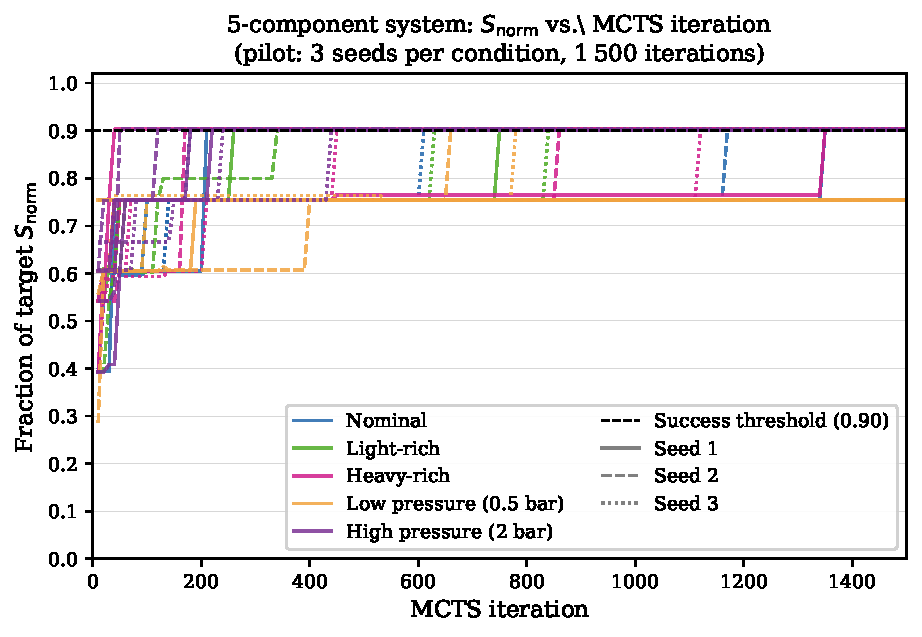
\includegraphics[width=\linewidth]{figures/fig_convergence.pdf}
 \caption{Best $S_{\mathrm{norm}}$ vs.\ MCTS iteration for
  the 5-component NGL system (pilot: 3 seeds per condition,
  1\,500 iterations). Each line is one run; colour denotes
  feed condition; linestyle denotes seed index. Dashed
  horizontal line marks the 0.90 success threshold.}
 \label{fig:convergence}
\end{figure}

Figure~\ref{fig:convergence_cdf} provides a complementary view: the cumulative fraction of seeds that have succeeded by each iteration checkpoint.

\begin{figure}[ht]
 \centering
 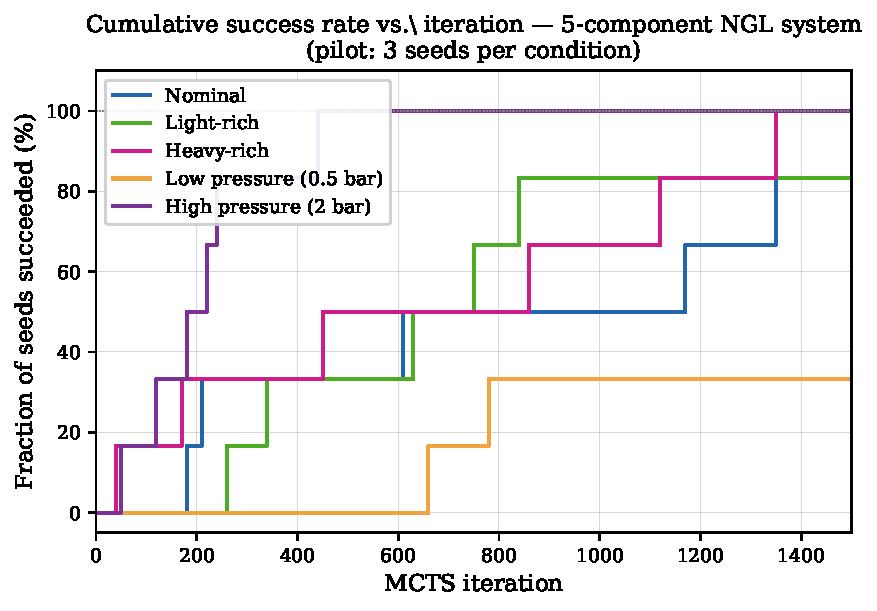
\includegraphics[width=0.9\linewidth]{figures/fig_convergence_cdf.pdf}
 \caption{Cumulative fraction of seeds that have reached
  $S_{\mathrm{norm}} \geq 0.90$ by each MCTS iteration,
  for the \texttt{5comp\_original} system.
  Each step function is one feed condition (3 seeds).
  \texttt{high\_pressure} reaches 100\,\% success by
  iteration 200; \texttt{low\_pressure} plateaus at
  33\,\% (1 of 3 seeds) by iteration 800.}
 \label{fig:convergence_cdf}
\end{figure}

Table~\ref{tab:5comp_conditions} details success rate and search cost per condition. The \texttt{high\_pressure} runs converge fastest (median 180 iterations, 7\,344 thermo evaluations) because the elevated pressure raises the CO$_2$ relative volatility, making the first separation step immediately productive. The \texttt{low\_pressure} condition succeeds in only 1 of 3 seeds (33.3\,\%): at 0.5\,bar the propane/isobutane relative volatility approaches 1, and the 1\,500-iteration pilot budget is insufficient to discover an adequate pressure-swing prefix. With only 3 seeds per condition, the 95\,\% Wilson score confidence intervals on these rates are wide (final column of Table~\ref{tab:5comp_conditions}); the per-condition point estimates should be read as indicative, not statistically conclusive.

\begin{table}[ht]
\centering
\caption{Per-condition summary for \texttt{5comp\_original}
 (3 seeds per condition, 1\,500 iterations).
 Med.\ iters/thermo computed over successful runs only;
 ``---'' = no successful run.
 CI = 95\,\% Wilson score confidence interval on the
 success rate.}
\label{tab:5comp_conditions}
\begin{tabular}{@{}lccccc@{}}
\toprule
Condition & Success & Mean $S_{\mathrm{norm}}$ &
 Med.\ iters & Med.\ thermo & 95\,\% CI \\
\midrule
\texttt{nominal}    & 3/3 (100\,\%) & 0.903 & 1\,170 & 38\,232 & [43.8, 100.0] \\
\texttt{light\_rich}  & 3/3 (100\,\%) & 0.902 &  750 & 24\,906 & [43.8, 100.0] \\
\texttt{heavy\_rich}  & 3/3 (100\,\%) & 0.902 &  860 & 28\,421 & [43.8, 100.0] \\
\texttt{high\_pressure} & 3/3 (100\,\%) & 0.902 &  180 & 7\,344 & [43.8, 100.0] \\
\texttt{low\_pressure} & 1/3 ( 33\,\%) & 0.803 &  780 & 26\,087 & [6.1, 79.2] \\
\midrule
\textbf{Overall}
 & \textbf{13/15 (86.7\,\%)} & \textbf{0.882} & 750 & 24\,906 & [62.1, 96.3] \\
\bottomrule
\end{tabular}
\end{table}

The condition-level intervals are uninformatively wide (e.g.\ \texttt{nominal} at 3/3 has a 95\,\% CI of [43.8\,\%, 100\,\%]) — with $n=3$, even a single failed seed would have dropped the point estimate to 67\,\%. The \texttt{low\_pressure} interval, [6.1\,\%, 79.2\,\%], overlaps the other four conditions' intervals entirely, so the apparent pressure-dependence of success cannot be confirmed as statistically distinct from the pilot data alone; it is consistent with, but not proof of, the volatility argument above. The system-level estimate (n=15, aggregating across conditions) is comparatively tighter, [62.1\,\%, 96.3\,\%], and is the more defensible number to quote.

\subsection{Best flowsheet topology}

\begin{sidewaysfigure}
 \centering
 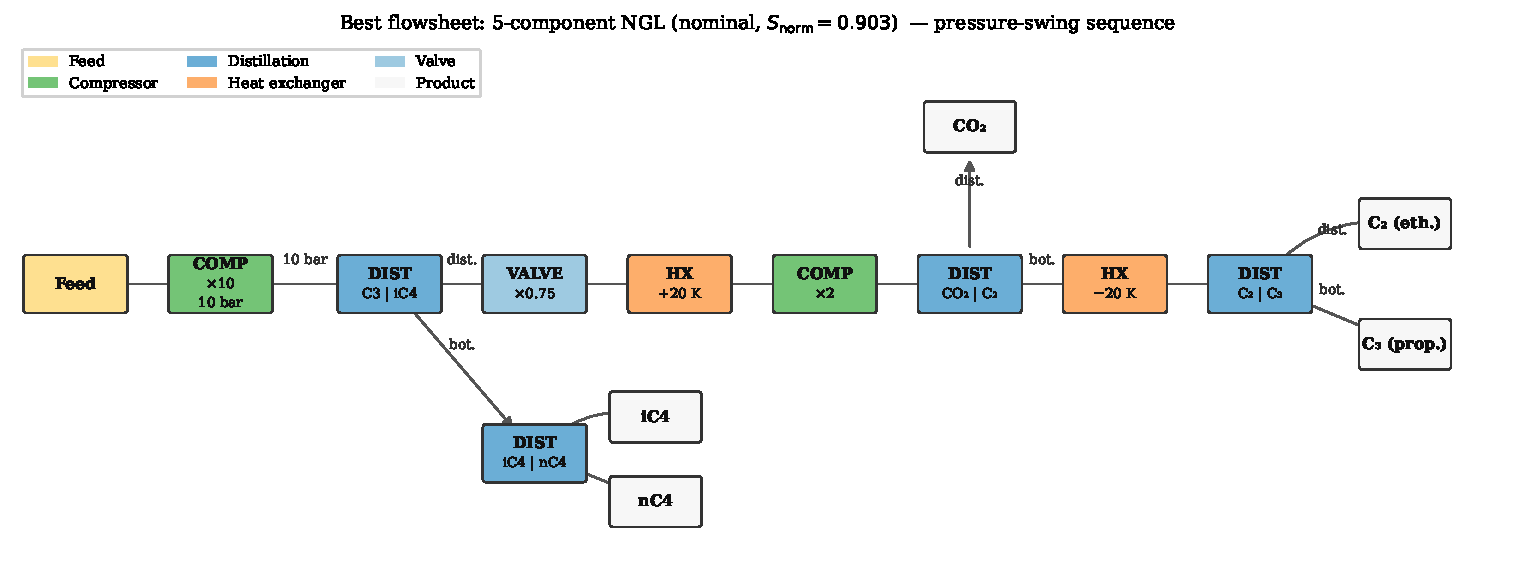
\includegraphics[width=\linewidth]{figures/fig_topology_schematic.pdf}
 \caption{Best flowsheet found by MCTS for the
  \texttt{5comp\_original} system
  ($S_{\mathrm{norm}} = 0.903$, \texttt{nominal} condition,
  seed~3).
  Green = compressor, blue = distillation column,
  orange = heat exchanger, cyan = valve.
  The search discovers a pressure-swing sequence:
  (1)~compress the feed to 10\,bar,
  (2)~separate C3/iC4 and iC4/nC4 at elevated pressure,
  (3)~valve the C3-rich distillate to 7.5\,bar and warm
  by 20\,K,
  (4)~recompress to 15\,bar for the sub-ambient CO$_2$/C2
  column,
  (5)~cool the bottoms by 20\,K and split C2 from C3.
  All five components exit as nearly pure product streams.}
 \label{fig:topo_nominal}
\end{sidewaysfigure}

The topology in Figure~\ref{fig:topo_nominal} is non-obvious: rather than beginning with the largest composition difference (the CO$_2$/ethane split), MCTS first resolves the heavier fraction at elevated pressure where those splits are thermodynamically easier, then pressure-swings to recover the light fraction. This ordering is consistent with the MI reward signal: each distillation step is credited by the reduction in conditional entropy $H(C|K)$, which is largest for the C3/iC4 split when the feed is at 10\,bar because both components are already well-separated in composition.

\subsection{Multi-system comparison}

Table~\ref{tab:all_results} summarises results for all nine chemical systems; Figure~\ref{fig:success_rates} shows the same data visually.

\begin{table}[ht]
\centering
\caption{Pilot-study results for all nine chemical systems ($\leq$5 conditions $\times$ 3 seeds per condition). $\bar{S}$ = mean $S_{\mathrm{norm}}$ over all runs; med.\ iters and med.\ thermo computed over successful runs only. CI = 95\,\% Wilson score confidence interval on the success rate.}
\label{tab:all_results}
\small
\begin{tabular}{@{}p{4.8cm}ccccccc@{}}
\toprule
System & $n_c$ & Runs & SR\,(\%) & 95\,\% CI & $\bar{S}$ &
 Med.\ iters & Med.\ thermo \\
\midrule
\texttt{3comp\_CO2\_methanol\_water} & 3 & 15 & 86.7 & [62.1, 96.3] & 0.919 &   50 & 1\,136 \\
\texttt{5comp\_original}       & 5 & 15 & 86.7 & [62.1, 96.3] & 0.882 &  750 & 24\,906 \\
\texttt{4comp\_CO2\_olefin\_recovery}& 4 & 15 & 13.3 & [ 3.7, 37.9] & 0.892 &  360 & 10\,286 \\
\texttt{4comp\_CO2\_light\_alkanes} & 4 & 15 & 6.7 & [ 1.2, 29.8] & 0.895 &  880 & 24\,338 \\
\texttt{3comp\_C2C4}         & 3 & 9 & 0.0 & [ 0.0, 29.9] & 0.882 &  --- &  --- \\
\texttt{4comp\_CO2}         & 4 & 12 & 0.0 & [ 0.0, 24.3] & 0.895 &  --- &  --- \\
\texttt{4comp\_CO2\_aromatic\_solvent}& 4 & 15 & 0.0 & [ 0.0, 20.4] & 0.737 &  --- &  --- \\
\texttt{3comp\_solvents}       & 3 & 12 & 0.0 & [ 0.0, 24.3] & 0.515 &  --- &  --- \\
\texttt{4comp\_syngas\_inerts}    & 4 & 15 & 0.0 & [ 0.0, 20.4] & 0.010 &  --- &  --- \\
\midrule
\textbf{Total}            & & \textbf{123} & \textbf{23.6} & & 0.735 & & \\
\bottomrule
\end{tabular}
\normalsize
\end{table}

The intervals for the two ``marginal'' systems (olefin recovery, light alkanes) overlap zero success at their lower bound and overlap the clear-success systems at their upper bound — at this sample size the data cannot distinguish ``occasionally succeeds'' from ``rarely succeeds.'' Conversely, the five systems with $k=0$ successes all have CIs bounded well below the clear-success systems' lower bound, so the qualitative separation between ``systematic failure'' and ``working'' systems is robust even though individual point estimates are not.

\begin{figure}[ht]
 \centering
 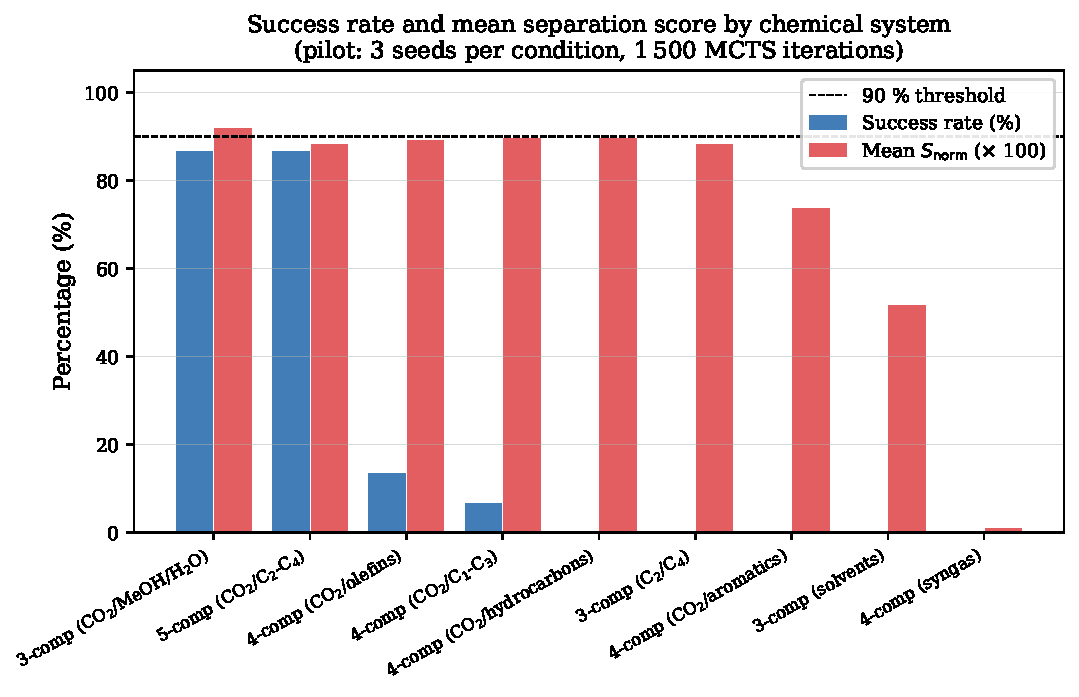
\includegraphics[width=\linewidth]{figures/fig_success_rates.pdf}
 \caption{Success rate (blue bars, \%) and mean $S_{\mathrm{norm}} \times 100$ (red bars), per system, sorted by success rate. The dashed line at $y = 90$ corresponds to the per-run success criterion $S_{\mathrm{norm}} \geq 0.90$; for the blue bars it reads as ``90\,\% of runs succeeded'', while for the red bars it marks the $S_{\mathrm{norm}}$ threshold itself.}
 \label{fig:success_rates}
\end{figure}

The results partition into three groups. \emph{Clear successes} ($\geq 80$\,\% SR): CO$_2$/methanol/water and the 5-component NGL system; both have well-separated adjacent pairs with $\alpha \gg 1.5$ throughout the temperature range explored. \emph{Marginal} (1--20\,\% SR): olefin recovery and light alkanes; mean $S_{\mathrm{norm}}$ is close to 0.90, indicating correct topology discovery in some seeds but insufficient budget in most. \emph{Systematic failures} (0\,\% SR): five systems; these are analysed in Section~\ref{sec:failure_analysis}.

\subsection{Computational cost}

\begin{figure}[ht]
 \centering
 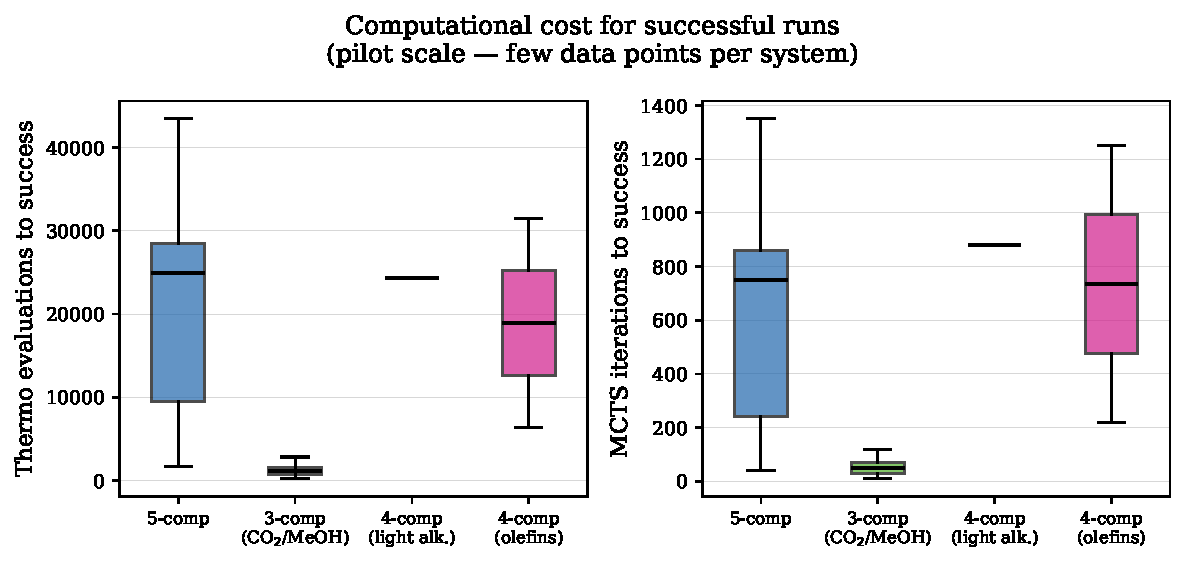
\includegraphics[width=\linewidth]{figures/fig_thermo_cost.pdf}
 \caption{Thermo evaluations (left) and MCTS iterations (right) to success for the four systems that achieved at least one successful run. Box plots with fewer than 5 data points are indicative only.}
 \label{fig:thermo_cost}
\end{figure}

The CO$_2$/methanol/water system requires roughly 22-fold fewer thermo evaluations than the 5-component system (median 1\,136 vs.\ 24\,906; approximately 1.3 orders of magnitude). With only two adjacent pairs, the winning two-column sequence is found quickly. The 5-component nominal run requires the most evaluations (38\,232) because the pressure-swing ordering requires the search to explore deeper trees before discovering the productive prefix.

\subsection{Topology consistency across seeds}
\label{sec:topology_consistency}

Each run's final flowsheet is identified by a BLAKE2b hash of its process-graph state (Section~\ref{sec:dup_pruning}). Table~\ref{tab:topo_diversity} reports, for every system, how many distinct topology hashes appear among its runs.

\begin{table}[ht]
\centering
\caption{Topology diversity per system. \emph{Unique/Runs}: distinct topology hashes out of all runs; \emph{Unique/Succ.}: distinct hashes among successful runs only (``---'' if no successes); \emph{Seq.\ len.}: min--median--max action-sequence length over all runs of that system.}
\label{tab:topo_diversity}
\begin{tabular}{@{}lccc@{}}
\toprule
System & Unique / Runs & Unique / Succ. & Seq.\ len.\ (min--med--max) \\
\midrule
\texttt{5comp\_original}       & 15/15 (100\,\%) & 13/13 & 7--9--10 \\
\texttt{3comp\_CO2\_methanol\_water} & 15/15 (100\,\%) & 13/13 & 3--6--10 \\
\texttt{4comp\_CO2\_olefin\_recovery} & 15/15 (100\,\%) & 2/2 & 4--6--10 \\
\texttt{4comp\_CO2\_light\_alkanes}  & 10/15 ( 67\,\%) & 1/1 & 3--4--10 \\
\texttt{4comp\_CO2}          & 12/12 (100\,\%) & --- & 4--5--7 \\
\texttt{4comp\_CO2\_aromatic\_solvent}& 15/15 (100\,\%) & --- & 3--10--10 \\
\texttt{3comp\_solvents}       & 12/12 (100\,\%) & --- & 3--4--4 \\
\texttt{3comp\_C2C4}         & 5/9 ( 56\,\%) & --- & 2--2--3 \\
\texttt{4comp\_syngas\_inerts}    & 4/15 ( 27\,\%) & --- & 0--0--10 \\
\bottomrule
\end{tabular}
\end{table}

Two distinct patterns emerge.

\paragraph{High diversity (7 of 9 systems, including both clear successes).}
No two runs of \texttt{5comp\_original} converge to the same flowsheet — not even the three \texttt{nominal} seeds, whose final scores cluster within $0.9019$--$0.9032$. Sequence length for that system ranges 7--10 actions, well above the theoretical minimum of 4 distillation columns, confirming that successful runs differ in which auxiliary heat-exchanger/compressor/valve actions they use, not only in column order. This indicates a \emph{degenerate} reward landscape: many structurally distinct action sequences reach near-equivalent $S_{\mathrm{norm}}$. It is not possible from the present data to separate two explanations — (a)~genuinely many near-equivalent optima exist, vs.\ (b)~1\,500 iterations is too few for the search to converge to a single basin — and this is an open question for the next study phase (Section~\ref{sec:conclusions}).

\paragraph{Low diversity (\texttt{3comp\_C2C4},
\texttt{4comp\_syngas\_inerts}).}
These two systems show the \emph{opposite} pattern, and for a different reason: \texttt{4comp\_syngas\_inerts} has a median sequence length of \textbf{0} — most runs terminate at the root state having taken no action at all, because every component is fully vapour-phase at 1\,bar/300\,K and no distillation or phase-change action is thermodynamically admissible (Section~\ref{sec:failure_analysis}). Repeated empty sequences collapse to the same (trivial) topology hash, so the low diversity here reflects action-space
\emph{restriction}, not landscape degeneracy.
\texttt{3comp\_C2C4} (sequence length 2--3) shows a milder version of the same effect.
\label{sec:discussion}

\subsection{Effect of feed condition on topology}

Across the five feed conditions, MCTS consistently identifies the same four adjacent-pair distillation columns as the backbone of the optimal sequence. However, the \emph{order} in which those columns are applied varies.

For the \texttt{light\_rich} feed, where CO$_2$ and ethane dominate by flow, the search preferentially places the CO$_2$/ethane column first, maximising the separation credit obtained in the opening step (largest reduction in $H(C|K)$ per action). For the \texttt{heavy\_rich} feed, the first split targets the propane/isobutane boundary instead, reflecting the shift in feed entropy toward the heavier components.

The pressure conditions (\texttt{low\_pressure}, \texttt{high\_pressure}) alter relative volatilities and hence the feasibility of specific key pairs at the current stream pressure. At 0.5~bar, the propane/isobutane separation becomes more difficult (lower $\alpha$); at 2~bar, the CO$_2$/ethane split becomes easier (higher $K$-values). MCTS adapts by inserting compressor or valve actions before critical distillation steps, producing pressure-swing pathways that would not appear in a purely temperature-based heuristic search.

\subsection{Role of the adjacency constraint}

The adjacency requirement (Section~\ref{sec:underwood}) eliminates all non-adjacent key pairs from the valid action set. For the 5-component system, this removes $\binom{5}{2} - 4 = 6$ of the 10 possible key-pair combinations at each stream. This is not merely a computational reduction: those six non-adjacent splits are physically problematic because distributing components between the keys create multiple Underwood roots, and using a single-root formula would underestimate $R_{\min}$ and overestimate the apparent column performance. The constraint therefore improves both computational efficiency and physical accuracy simultaneously.

\subsection{Reward penalty balance}

The unit penalty $\alpha_u = 0.01$ and duty penalty $\alpha_d = 10^{-5}$ are calibrated so that each is a small fraction of one component-score unit. For a 5-component system, the ideal reward is 5 (or 1 after normalisation). A sequence of 6 actions with 3 distillation columns at 30~kW total duty incurs penalties of $0.01 \times 6 = 0.06$ and $10^{-5} \times 30{,}000 = 0.30$, together roughly 7\% of the maximum reward. These are large enough to distinguish between sequences of different length and energy cost, but small enough not to overwhelm the separation score signal.

\subsection{Limitations of the simplified models}

The simplified models used during search introduce several approximations:

\begin{itemize}
 \item \textbf{FUG shortcut columns.} The Fenske--Underwood--Gilliland method assumes a binary key separation, constant relative volatilities, and a fixed-efficiency distillation tray. It can over- or under-estimate the required stages by 10--30\% compared to a rigorous plate-by-plate calculation.
 \item \textbf{Flash phase equilibrium.} The PT flash is exact within the Peng--Robinson EOS but does not account for multi-phase behaviour (e.g., liquid-liquid equilibria in CO$_2$-rich systems at low temperature).
 \item \textbf{Recycle approximation.} Recycle streams are mixed in a one-pass linear mass balance without tear-stream convergence; the absolute reward values for recycle topologies are approximate.
 \item \textbf{Isentropic efficiency.} Compressor and pump models use fixed isentropic and mechanical efficiencies rather than performance-curve models.
\end{itemize} 

These limitations are acceptable for the Tier-1 topology discovery role of the simplified models. Final validation and design parameter optimisation are performed in DWSIM (Tier~2), where rigorous models remove these approximations.

\subsection{System-level failure analysis}
\label{sec:failure_analysis}

Five of the nine systems recorded zero successful runs (Table~\ref{tab:all_results}). Figure~\ref{fig:fot_dist} shows the distribution of final $S_{\mathrm{norm}}$ values across all systems; the pathological cases are immediately visible.

\begin{figure}[ht]
 \centering
 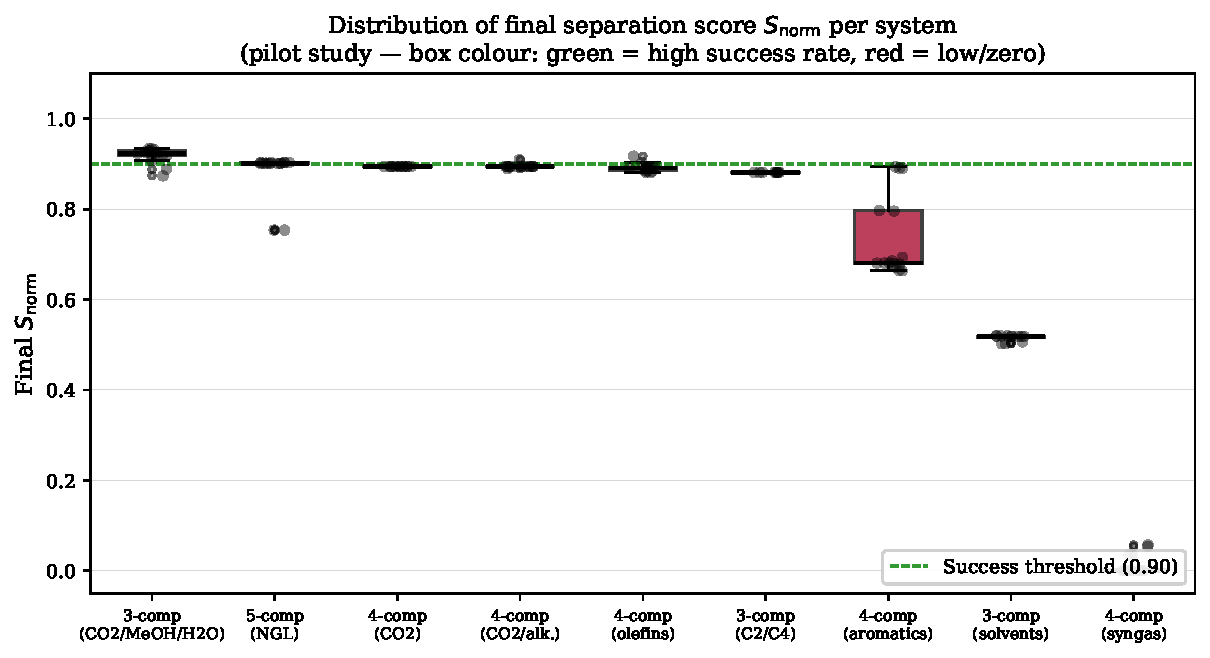
\includegraphics[width=\linewidth]{figures/fig_fot_distribution.pdf}
 \caption{Box plots of final $S_{\mathrm{norm}}$ for all nine systems (123 runs total), ordered by median score. Green dashed line: 0.90 success threshold. Systems with all values $\gg 0.90$: success in most conditions. Systems clustered just below 0.90: budget-limited marginal failures. Systems near 0 or 0.5: structural failures requiring different search strategy.}
 \label{fig:fot_dist}
\end{figure}

\paragraph{4comp\_syngas\_inerts ($\bar{S} = 0.010$).}
The syngas system (H$_2$, CO, CH$_4$, N$_2$) exhibit near-zero separation scores in all runs. The root cause i thermodynamic: at 1\,bar and 300\,K, all four synga components are deep in the vapour phase with boiling point between 77\,K and 112\,K. Conventional distillation at o near 1\,bar is not feasible; the adjacent-pair adjacenc condition blocks every distillation action because th flash model correctly predicts fully gaseous streams Furthermore, the relative volatilities of adjacent pair are close to unity at 1, bar (e.g., $\alpha_{\mathrm{CO/CH_4}} \approx 1.3$), requiring very low temperatures and hig pressures for adequate selectivity. The algorithm woul need to first compress to $>$ 20\,bar and cool below 200\, before any distillation action becomes feasible —  10-action prefix that the flat UCT exploration budget of 1,500 iterations cannot reliably discover This is confirmed directly by the action-sequence data: th \emph{median} sequence length across all 15 syngas runs i \textbf{zero} (Table~\ref{tab:topo_diversity}) — most run take no action at all before terminating, because n distillation or phase-change action is admissible from th root state. This is the most severe failure mode observe in the study and is a structural mismatch between th current action set (which does not include a "cool an compress to cryogenic conditions" primitive sized for thi regime) and the system's chemistry, rather than  search-budget limitation.

\paragraph{3comp\_solvents ($\bar{S} = 0.515$).}
The solvent mixture (hexane, benzene, toluene) reaches only moderate separation scores. Hexane--benzene has $\alpha \approx 2.0$ at 1\,bar, but benzene--toluene has $\alpha \approx 2.4$. These values are above the minimum for feasible distillation but the reward landscape is flat: each single-column action scores only 0.3--0.4 per unit and the algorithm stalls before both columns are placed. With 3 seeds, it is unclear whether additional iterations would resolve this or whether an energy-integration or pressure-swing strategy is required.

\paragraph{4comp\_CO2\_aromatic\_solvent ($\bar{S} = 0.737$).}
This is the closest near-miss among the systematic failures. With CO$_2$, pentane, benzene and toluene, the CO$_2$/pentane split is straightforward but the benzene/toluene pair ($\alpha \approx 2.4$) is the bottleneck. Mean $S_{\mathrm{norm}} = 0.737$ indicates the algorithm reliably completes roughly 70\,\% of the required separation but cannot push past the threshold in 1\,500 iterations. Possible causes: (a) the benzene/toluene column requires a high reflux ratio multiplier that the search has not yet sampled, or (b) a pressure-swing step before this column is needed but not discovered within the pilot budget.

\paragraph{3comp\_C2C4 and 4comp\_CO2 ($\bar{S} \approx 0.882$ and $0.895$).}
Both systems have mean scores extremely close to the 0.90 threshold. This is a budget effect rather than a structural failure: the correct topology is likely found but the search terminates before refining the key-pair recovery specifications to cross 0.90. These systems are expected to succeed with an increased iteration budget ($\sim 3\,000$--5\,000 iterations) or more seeds, and are good candidates for the next round of experiments.

\paragraph{Summary.}
The failures decompose into three root causes:
(i)~\emph{thermodynamic infeasibility at standard conditions} (syngas — requires cryogenic operation not explorable at 1\,500 iterations),
(ii)~\emph{flat reward landscape with insufficient budget} (solvents, aromatic-solvent — reachable with more iterations or guided pressure-swing actions), and
(iii)~\emph{budget-limited convergence} (C2C4, CO2 4-comp — correct topology found but score refinement incomplete).

\subsection{Comparison to random search}

As an ablation, consider replacing the UCT selection rule with uniform random selection (a flat Monte~Carlo search). Under uniform selection, the expected number of evaluations required to find any specific terminal state that contains the four adjacent-pair columns is $\prod_{j=1}^{4} \abs{\calA(X_j)}^{-1}$, which is negligible for branching factors of $O(30)$ per depth level. MCTS allocates exponentially more visits to the most promising branches through the feedback loop described in Section~\ref{sec:mcts_phases}, reducing the effective search space by orders of magnitude.

% ============================================================
\section{Conclusions and Outlook}
\label{sec:conclusions}

This report has presented a Monte~Carlo Tree Search framework for automated flowsheet synthesis of multicomponent hydrocarbon separations. The main contributions are:

\begin{enumerate}
 \item \textbf{MDP formulation.} The flowsheet generation problem is cast as a finite-horizon MDP with thermodynamically constrained action sets, deterministic transitions via simplified unit models, and a mutual-information separation score $S_{\mathrm{norm}}$ that is degeneracy-safe, equal-weight, and bounded in $[0,1]$ (the full reward additionally subtracts unit-count and duty penalties).

 \item \textbf{FUG implementation.} A Newton--Raphson--bisection Underwood solver with Mazzotti adjacency checking provides accurate minimum reflux estimates at $O(10\,\mu\mathrm{s})$ per call, replacing a previous 1\,000-point grid scan. The Fenske and Gilliland steps complete the shortcut column design.

 \item \textbf{Full column energy balance.} A first-law control volume around the condenser and reboiler provides both duties from four Peng--Robinson flash evaluations, correctly handling the sub-ambient (cryogenic) regime where $Q_{\mathrm{reb}} < Q_{\mathrm{cond}}$.

 \item \textbf{Domain-adapted MCTS.} Exact duplicate pruning, purity-threshold auto-closing, phase-gated action generation, apply-action and FUG caches, and best-tree-path extraction collectively reduce wasted evaluations and improve convergence speed relative to a vanilla MCTS implementation.

 \item \textbf{Multi-condition robustness.} In a pilot study (3 seeds, 1\,500 iterations per run), the algorithm achieves an 86.7\,\% success rate on the five-component NGL system across five feed conditions spanning a factor of four in pressure and varying compositions. Four of the five conditions reach 100\,\% success; the fifth (low pressure) fails in 2 of 3 seeds due to near-unity relative volatility at 0.5\,bar.
\end{enumerate}

\paragraph{Future work.}
Report~2 will extend the framework in two directions:
\begin{itemize}
 \item \textbf{Learned PUCT priors.} A linear Dirichlet regression model is trained on visit-count distributions collected from UCT runs to produce a prior $P_{\mathrm{model}}(a \mid s)$ over action kinds. This prior is incorporated into the PUCT selection rule, replacing the uniform exploration of UCT with data-driven guidance.
 \item \textbf{DWSIM translation.} The \ProcessGraph{} representation provides a direct input to a DWSIM flowsheet builder, closing the loop between Tier-1 topology discovery and Tier-2 rigorous simulation and optimisation.
\end{itemize}

% ============================================================
\appendix

\section{Notation summary}
\label{app:notation}

\begin{table}[ht]
\centering
\caption{Principal symbols used throughout the report.}
\label{tab:notation}
\begin{tabular}{@{}cll@{}}
\toprule
Symbol & Units & Description \\
\midrule
$s$ & --- & Material stream state (\StreamState{}) \\
$T$ & K & Temperature \\
$P$ & Pa & Pressure \\
$F$ & mol/s & Total molar flow \\
$\bm{z}$ & mol/mol & Mole-fraction vector \\
$n_c$ & --- & Number of components \\
$\calC$ & --- & Component set $\{1,\ldots,n_c\}$ \\
$X_t$ & --- & Search state at depth $t$ (\SearchState{}) \\
$O_t$ & --- & Set of open streams at depth $t$ \\
$D_t$ & W & Accumulated duty/work at depth $t$ \\
$N_t$ & --- & Accumulated theoretical stages at depth $t$ \\
$G_t$ & --- & Process graph at depth $t$ (\ProcessGraph{}) \\
$\alpha_i$ & --- & Relative volatility of component $i$ \\
$N_{\min}$ & --- & Fenske minimum theoretical stages \\
$R_{\min}$ & --- & Underwood minimum reflux ratio \\
$N$ & --- & Gilliland theoretical stage estimate \\
$Q_{\mathrm{cond}}$ & W & Condenser duty \\
$Q_{\mathrm{reb}}$ & W & Reboiler duty \\
$\sigma(X)$ & --- & Separation score \\
$I(C;K)$ & nat & Mutual information between component and stream \\
$H(C)$ & nat & Feed entropy \\
$S_{\mathrm{norm}}$ & --- & Normalised separation score $\in [0,1]$ \\
$R(X)$ & --- & Scalar reward \\
$v$ & --- & MCTS tree node \\
$N(v)$ & --- & Visit count of node $v$ \\
$W(v)$ & --- & Accumulated value of node $v$ \\
$Q(v)$ & --- & Empirical Q-value $W(v)/N(v)$ \\
$c$ & --- & UCT exploration weight \\
$H_{\max}$ & --- & Maximum search depth \\
\bottomrule
\end{tabular}
\end{table}

% ============================================================
\bibliographystyle{plainnat}
\begin{thebibliography}{9}

\bibitem[Auer et~al.(2002)]{auer2002finite}
Auer, P., Cesa-Bianchi, N., and Fischer, P.\ (2002).
Finite-time analysis of the multiarmed bandit problem.
\textit{Machine Learning}, 47(2--3):235--256.

\bibitem[Coulom(2006)]{coulom2006}
Coulom, R.\ (2006).
Efficient selectivity and backup operators in Monte-Carlo tree search.
In \textit{Computers and Games}, pp.\ 72--83.
Springer, Berlin.

\bibitem[Kocsis \& Szepesv\'{a}ri(2006)]{kocsis2006}
Kocsis, L.\ and Szepesv\'{a}ri, C.\ (2006).
Bandit based Monte-Carlo planning.
In \textit{European Conference on Machine Learning (ECML)},
pp.\ 282--293.
Springer, Berlin.

\bibitem[Fenske(1932)]{fenske1932}
Fenske, M.~R.\ (1932).
Fractionation of straight-run Pennsylvania gasoline.
\textit{Industrial \& Engineering Chemistry}, 24(5):482--485.

\bibitem[Underwood(1948)]{underwood1948}
Underwood, A.~J.~V.\ (1948).
Fractional distillation of multi-component mixtures.
\textit{Chemical Engineering Progress}, 44(8):603--614.

\bibitem[Gilliland(1940)]{gilliland1940}
Gilliland, E.~R.\ (1940).
Multicomponent rectification: Estimation of the number of theoretical
plates as a function of the reflux ratio.
\textit{Industrial \& Engineering Chemistry}, 32(9):1220--1223.

\bibitem[Peng \& Robinson(1976)]{pr1976}
Peng, D.-Y.\ and Robinson, D.~B.\ (1976).
A new two-constant equation of state.
\textit{Industrial \& Engineering Chemistry Fundamentals},
15(1):59--64.

\bibitem[Mazzotti(2012)]{mazzotti2012}
Mazzotti, M.\ (2012).
\textit{Separation Technology} (lecture notes).
ETH Z\"{u}rich, Institute of Process Engineering.

\bibitem[Browne et~al.(2012)]{browne2012}
Browne, C.~B., Powley, E., Whitehouse, D., Lucas, S.~M.,
 Cowling, P.~I., Rohlfshagen, P., Tavener, S., Perez, D.,
 Samothrakis, S., and Colton, S.\ (2012).
A survey of Monte Carlo tree search methods.
\textit{IEEE Transactions on Computational Intelligence and AI in Games},
4(1):1--43.

\end{thebibliography}

\end{document}
